\newpage
\section{HÀM SỐ VÀ ĐỒ THỊ}
\subsection{LÝ THUYẾT CẦN NHỚ}
\subsubsection{Tính đơn điệu của hàm số}
\indam{Định nghĩa:}
\begin{boxdn}
	Giả sử $x$ và $y$ là hai đại lượng biến thiên và $x$ nhận giá trị thuộc tập số $\mathscr{D}$.\\
	Nếu với mỗi giá trị $x$ thuộc $\mathscr{D}$, ta xác định được một và chỉ một giá trị tương ứng $y$ thuộc tập hợp số thực $\mathbb{R}$ thì ta có một hàm số.\\
	Ta gọi $x$ là biến số và $y$ là hàm số của $x$.\\
	Tập hợp $\mathscr{D}$ được gọi là tập xác định của hàm số.\\
	Tập hợp $T$ gồm tất cả các giá trị $y$ (tương ứng với $x$ thuộc $\mathscr{D}$) gọi là tập giá trị của hàm số.
\end{boxdn}

\begin{khung4}{Ghi nhớ 1}
	\begin{itemize}
		\item Khi một hàm số được cho bằng công thức mà không chỉ rõ tập xác định thì ta quy ước: \textit{Tập xác định của hàm số $y=f(x)$ là tập hợp tất cả các số thực $x$ sao cho biểu thúc $f(x)$ có nghĩa.}
		
		\item Một hàm số có thể được cho bởi hai hay nhiều công thức. Chẳng hạn, xét hàm số
		\[f(x)= \heva{&-3x+5 & \text { với } x \leq 1 \\ & 2 x^2 & \text { với } x>1}\]
		nghĩa là với $x \leq 1$ thì $f(x)=-3x+5$; với $x>1$ thì $f(x)=2x^2$.
	\end{itemize}
\end{khung4}

\subsubsection{Đồ thị hàm số}
\begin{boxdn}
	Cho hàm số $y=f(x)$ có tập xác định $\mathscr{D}$.\\
	Trên mặt phẳng toạ độ $Oxy$, đồ thị $(C)$ của hàm số là tập hợp tất cả các điểm $M(x;y)$ với $x \in \mathscr{D}$ và $y=f(x)$.\\
	Vậy $(C)=\{M(x;f(x)) \mid x \in \mathscr{D}\}$.
\end{boxdn}
\begin{khung4}{Ghi nhớ 2}
	Điểm $M\left(x_{M};y_{M}\right)$ thuộc đồ thị hàm số $y=f(x)$ khi và chỉ khi $x_{M} \in \mathscr{D}$ và $y_{M}=f\left(x_{M}\right)$.
\end{khung4}
\subsubsection{Tính đơn điệu của hàm số}
\begin{boxdn}
	Với hàm số $y=f(x)$ xác định trên khoảng $(a;b)$, ta nói
	\begin{itemize}
		\item Hàm số đồng biến trên khoảng $(a;b)$ nếu
		\[\forall x_{1}, x_{2} \in(a ; b), x_{1}<x_{2} \Rightarrow f\left(x_{1}\right)<f\left(x_{2}\right).\]
		\item Hàm số nghịch biến trên khoảng $(a;b)$ nếu
		\[\forall x_{1}, x_{2} \in(a ; b), x_{1}<x_{2} \Rightarrow f\left(x_{1}\right)>f\left(x_{2}\right).\]
	\end{itemize}
\end{boxdn}
\begin{khung4}{Ghi nhớ 3}
	Khi hàm số đồng biến (tăng) trên khoảng $(a;b)$ thì đồ thị của nó có dạng đi lên từ trái sang phải. Ngược lại, khi hàm số nghịch biến (giảm) trên khoảng $(a;b)$ thì đồ thị của nó có dạng đi xuống từ trái sang phải.
\end{khung4}

%-------------------------------------------------------------------------------------------------------------
\subsection{PHÂN LOẠI VÀ PHƯƠNG PHÁP GIẢI TOÁN}
\begin{dang}{Tìm tập xác định của hàm số}
	Phương pháp giải
	\begin{listEX}[1]
		\item [\ding{172}] Hàm số  $y=\dfrac{1}{A}$: Điều kiện là $A\neq 0$.
		\item [\ding{172}] Hàm số  $y=\sqrt{A}$: Điều kiện là $A\geq 0$.
		\item [\ding{172}] Hàm số $y=\dfrac{1}{\sqrt{A}}$: Điều kiện là $A>0$.
	\end{listEX}
\end{dang}

\begin{vd}%[0D3N1-2]%[Dự án đề cương 2025]%[Mui Doan]
	Tìm tập xác định của các hàm số sau
	\begin{listEX}[2]
		\item $f(x)=\dfrac{1}{2x-6}$.
		\item $f(x)=\sqrt{5-x}$.
		\item $f(x)=\sqrt{-5x+3}$.
		\item $f(x)=2+\dfrac{1}{x+3}$.
	\end{listEX}
	\loigiai{
		\begin{enumerate}
			\item Điều kiện $2x-6 \neq 0$, tức là khi $x \neq 3$.\\
			Vậy tập xác định của hàm số này là $\mathscr{D}=\mathbb{R}\setminus\{3\}$.
			\item Điều kiện $5-x \geq 0$, tức là khi $x \leq 5$.\\
			Vậy tập xác định của hàm số này là $\mathscr{D}=(-\infty;5]$.
			\item Điều kiện $-5x+3 \geq 0$, tức là khi $x \leq \dfrac{3}{5}$.\\
			Vậy tập xác định của hàm số này là $\mathscr{D}=\left(-\infty;\dfrac{3}{5}\right]$.
			\item Điều kiện $x+3 \neq 0$, tức là khi $x \neq -3$.\\
			Vậy tập xác định của hàm số này là $\mathscr{D}=\mathbb{R}\setminus\{-3\}$.
		\end{enumerate}
}
\end{vd}
\begin{vd}%[0D3H1-2]
	[10 HKI NH24-25-SGD - BẮC NINH]
	Tìm tập xác định của các hàm số sau
	\begin{enumerate}
		\item $y = \dfrac{2x^2 - 3}{x + 5}$.
		\item $y = \sqrt{x^2 + 1}$.
		\item $y = \sqrt{2 - x} - \dfrac{2}{\sqrt{x + 1}}$.
	\end{enumerate}
	\loigiai{
		\begin{enumerate}
			\item $y=\dfrac{2x^2-3}{x+5}$.\\
			Hàm số xác định khi $x+5\ne 0\Leftrightarrow x\ne -5$.\\ 
			Tập xác định $\mathscr{D}=\mathbb{R}\setminus \{-5\}$.
			\item $y=\sqrt{x^2+1}$.\\
			Hàm số xác định khi $x^2+1\ge 0$.\\
			Vì $x^2\ge 0$ với mọi $x\in \mathbb{R}$ nên $x^2+1\ge 0$ với mọi $x\in \mathbb{R}$.\\
			Tập xác định: $\mathscr{D}=\mathbb{R}$.
			\item $y=\sqrt{2-x}-\dfrac{2}{\sqrt{x+1}}$.\\
			Hàm số xác định 
			\begin{eqnarray*}
				&&\Leftrightarrow \heva {& 2-x\ge 0\\&x+1> 0}\\
				&&\Leftrightarrow \heva {& x\le 2\\&x> -1}\\
				&&\Leftrightarrow -1<x\le 2.
			\end{eqnarray*}
			Tập xác định: $\mathscr{D}=\left(-1;2\right]$.
		\end{enumerate}
	}
\end{vd}
\begin{vd}%[0D3H1-2]
	[THPT HỒ THỊ BI TP. HCM - Lớp 10 - GK1]
	Tìm tập xác định $\mathscr{D}$ của hàm số $y = \dfrac{x+1}{(x-3)\sqrt{2x+1}}$.
	\loigiai{Hàm số xác định 
		\begin{eqnarray*}
			&&\Leftrightarrow \heva {&x-3\ne 0\\&2x+1>0}\\
			&&\Leftrightarrow \heva {&x\ne 3\\&x> -\dfrac{1}{2}}\\
			&&\Leftrightarrow x\in \left( -\dfrac{1}{2}; +\infty \right) \setminus \{3\}.
		\end{eqnarray*}
		Tập xác định: $\mathscr{D}=\left( -\dfrac{1}{2}; +\infty \right) \setminus \{3\}$.
	}
\end{vd}

\begin{dang}{Xác định điểm thuộc đồ thị, tập xác định và tập giá trị từ đồ thị}
	Phương pháp
	\begin{itemize}
		\item  Điểm thuộc đồ thị: Thay tọa độ điểm vào công thức hàm số (nếu có) hoặc kiểm tra trực tiếp trên đồ thị xem điểm đó có nằm trên đường cong (hoặc các điểm rời rạc) của đồ thị hay không.
		\item  Tập xác định: Chiếu đồ thị lên trục hoành để tìm miền giá trị của $x$.
		\item  Tập giá trị: Chiếu đồ thị lên trục tung để tìm miền giá trị của $y$.
	\end{itemize}
\end{dang}

\begin{vd}%[0D3N1-4]%[Dự án đề cương 2025]%[Mui Doan]
	\begin{enumerate}
		\item 
		\immini{
			Cho hàm số $y=f(x)=\dfrac{1}{8} x^{2}$ xác định trên $D=[-3 ; 5]$ có đồ thị $(C)$ như hình bên. Điểm $A(4;f(4))$ có thuộc đồ thị $(C)$ không?
				}{
			\begin{tikzpicture}[scale=0.8, font=\footnotesize, line join=round, line cap=round, >=stealth]
				\draw[->] (-3.5,0)--(5.5,0) node[above]{$x$};
				\draw[->] (0,-1)--(0,3.5) node[right]{$y$};
				\draw[fill=black] (0,0) circle (1pt) node[below left] {$O$};
				\draw [domain=-3:5, samples=100] plot (\x, {1/8*(\x)^2});
				\draw[dashed] (0,2)--(4,2)--(4,0)
				(-2.5,25/32)--(-2.5,0);
				\draw[fill=black] (-3,9/8) circle (1pt);
				\draw[fill=black] (5,25/8) circle (1pt);
				\draw[fill=black] (4,2) circle (1pt) node[above left]{$A$};
				\draw[fill=black] (-2.5,25/32) circle (1pt) node[above right]{$B$};
				\draw[fill=black] (-2.5,0) circle (1pt) node[above left=0 and -0.1]
				{\scriptsize $x_B$};
				\foreach \i in {-3,-2,-1,1,2,3,4,5}
				\draw[fill=black] (\i,0)node[below]{$\i$}circle(1pt);
				\foreach \i in {1,2,3}
				\draw[fill=black] (0,\i)node[left]{$\i$}circle(1pt);
				\node[above right] at (4.5,2){$(C):y=\dfrac{1}{8}x^2$};
			\end{tikzpicture}
		}
		\item Lấy điểm $B$ tuỳ ý trên đồ thị $(C)$. Nêu nhận xét về hoành độ của điểm $B$.
	\end{enumerate}
	\loigiai{
		\begin{enumerate}
			\item Vì $4 \in[-3;5]$ nên điểm $A$ có hoành độ bằng $4$ và có tung độ $y=\dfrac{1}{8} \cdot 4^2=2$ là điểm thuộc đồ thị $(C)$.\\
			\item Khi lấy điểm $B$ tuỳ ý trên đồ thị $(C)$ thì hoành độ $x_{B}$ của điểm này thuộc tập xác định $D$, nghĩa là $-3 \leq x_{B} \leq 5$.
		\end{enumerate}
	}
\end{vd}
\begin{vd}%[0D3N1-2]%[Dự án đề cương 2025]%[Mui Doan]
	Tìm tập xác định, tập giá trị của hàm số có đồ thị như hình vẽ
	\begin{center}
		\begin{tikzpicture}[scale=0.6, font=\footnotesize, line join=round, line cap=round, >=stealth]
			\draw [->] (-5,0)--(11,0) node[below]{$x$};
			\draw [->] (0,-3)--(0,8) node[right]{$y$};
			\draw[fill=black] (0,0) circle(1pt) node[below left]{$O$};
			\draw[opacity=0.1] (-5,-3) grid (11,8);
			\clip (-5,-3) rectangle (11,8);
			\draw[name path=c1,smooth, samples=300, domain=-1:1] plot (\x,{-0.5*(\x)^2+1.5*(\x)+3});
			\draw[name path=c2,smooth, samples=300, domain=1:5] plot (\x,{-(1/6)*(\x)^2-0.5*(\x)+14/3});
			\draw (5,-2)--(9,6);
			\foreach \i in {-4,-2,2,4,6,8} \draw [fill=black] (\i,0) circle(1pt) node[below]{$\i$};
			\foreach \j in {-2,2,4,6} \draw [fill=black] (0,\j) circle(1pt) node[left]{$\j$};
			\draw [fill=black](-1,1) circle(1pt);
			\draw [fill=black](9,6) circle(1pt);
		\end{tikzpicture}
	\end{center}
	\loigiai{
		Dựa vào đồ thị của hàm số, ta thấy hàm số có tập xác định $\mathscr{D}=[-1;9]$ và tập giá trị $T=[-2;6]$.
	}
\end{vd}
\begin{dang}{Xét tính đồng biến, nghịch biến của hàm số}
	Phương pháp giải
	\begin{itemize}
		\item  Sử dụng định nghĩa: Lấy hai giá trị $x_1$, $x_2$	bất kỳ thuộc khoảng cần xét sao cho $x_1<x_2$.\\
		So sánh $f(x _1)$  và $f(x_2)$.
		\begin{itemize}
			\item Nếu $f(x _1)<f(x_2)$, hàm số đồng biến.
			\item Nếu $f(x _1)>f(x_2)$, hàm số nghịch biến.
		\end{itemize}
		\item  Sử dụng đồ thị: Quan sát dạng của đồ thị trên các khoảng.
	\end{itemize}
\end{dang}

\begin{vd}%[0D3H1-5]%[Dự án đề cương 2025]%[Mui Doan]
	\immini{
		Xét tính đồng biến, nghịch biến của các hàm số sau trên tập xác định hoặc trên khoảng được chỉ định
		\begin{enumerate}
			\item $y=3x-1$;
			\item $y=x^{2}$ trên khoảng $(-\infty;0)$;
			\item Hàm số có đồ thị như hình bên.
		\end{enumerate}
	}{
		\begin{tikzpicture}[scale=0.6, font=\footnotesize, line join=round, line cap=round, >=stealth]
			\draw[->] (-5,0)--(9,0) node[above]{$x$};
			\draw[->] (0,-3)--(0,5) node[right]{$y$};
			\draw[very thin,step=1cm,color=gray,dashed] (-5,-3)grid(9,5);
			\draw (-3,-2)--(-2,2)--(5,1.2)--(7,3);
			\foreach \i/\j in {-3/-2,7/3}
			\draw[fill=black] (\i,\j)circle(2pt);
			\foreach \i in {-4,-2,2,4,6,8}
			\draw[fill=black] (\i,0)node[below]{$\i$}circle(1pt);
			\foreach \i in {-2,2,4}
			\draw[fill=black] (0,\i)node[above right=-0.15 and 0]{$\i$}circle(1pt);
			\draw[fill=black] (0,0) circle (1pt) node[below left] {$O$};
		\end{tikzpicture}
	}
	\loigiai{
		\begin{enumerate}
			\item Xét hàm số $y=f(x)=3 x-1$. Hàm số này xác định trên $\mathbb{R}$.\\
			Lấy $x_{1}, x_{2}$ là hai số tuỳ ý sao cho $x_{1}<x_{2}$, ta có
			\[x_{1}<x_{2} \Rightarrow 3 x_{1}<3 x_{2} \Rightarrow 3 x_{1}-1<3 x_{2}-1 \Rightarrow f\left(x_{1}\right)<f\left(x_{2}\right).\]
			Vậy hàm số đồng biến (tăng) trên $\mathbb{R}$.
			
			\item Xét hàm số $y=x^{2}$ trên khoảng $(-\infty;0)$.\\	
			Lấy $x_{1}, x_{2}$ tuỳ ý sao cho $x_{1}<x_{2}$, ta có \[f\left(x_{1}\right)-f\left(x_{2}\right)=x_{1}^{2}-x_{2}^{2}=\left(x_{1}+x_{2}\right)\left(x_{1}-x_{2}\right).\]
			Do $x_{1}<x_{2}$ nên $x_{1}-x_{2}<0$ và do $x_{1}, x_{2} \in(-\infty;0)$ nên $x_{1}+x_{2}<0$. \\
			Từ đây suy ra $f\left(x_{1}\right)-f\left(x_{2}\right)>0$ hay $f\left(x_{1}\right)>f\left(x_{2}\right)$.\\
			Vậy hàm số nghịch biến (giảm) trên khoảng $(-\infty;0)$.
			
			\item Từ đồ thị, ta thấy hàm số xác định trên $[-3;7]$.
			\begin{itemize}
				\item Trên khoảng $(-3;-2)$, đồ thị có dạng đi lên từ trái sang phải nên hàm số này đồng biến trên khoảng $(-3;-2)$.
				\item Trên khoảng $(-2;5)$, đồ thị có dạng đi xuống từ trái sang phải nên hàm số này nghịch biến trên khoảng $(-2;5)$.
				\item Trên khoảng $(5;7)$, đồ thị có dạng đi lên từ trái sang phải nên hàm số này đồng biến trên khoảng $(5;7)$.
			\end{itemize}
		\end{enumerate}
	}
\end{vd}
\begin{vd}%[0D3H1-5]%[Dự án đề cương 2025]%[Mui Doan]
	Tìm các khoảng đồng biến, nghịch biến của các hàm số sau
	\begin{enumerate}[a)]
		\item $f(x)=-5x+2$;
		\item $f(x)=-x^2$.
	\end{enumerate}
	\loigiai{
		\begin{enumerate}[a)]
			\item Xét hàm số $f(x)=-5x+2$. Hàm số này có tập xác định là $\mathbb{R}$.\\
			Lấy $x_1$, $x_2$ là hai số tùy ý sao cho $x_1<x_2$, ta có $$x_1<x_2\Rightarrow -5x_1>-5x_2\Rightarrow -5x_1+2>-5x_2+2\Rightarrow f(x_1)>f(x_2).$$
			Vậy hàm số $f(x)=-5x+2$ nghịch biến trên $\mathbb{R}$. 
			\item Xét hàm số $f(x)=-x^2$. Hàm số này có tập xác định là $\mathbb{R}$.\\
			Lấy $x_1$, $x_2$ tùy ý sao cho $x_1<x_2$, ta có $f(x_1)-f(x_2)=-x_1^2+x_2^2=-(x_1-x_2)(x_1+x_2)$.
			\begin{itemize}
				\item Xét trên khoảng $(-\infty;0)$:\\
				Vì $x_1<x_2$ nên $x_1-x_2<0$ và do $x_1$, $x_2\in (-\infty;0)$ nên $x_1+x_2<0$.\\
				Từ đó suy ra $(x_1-x_2)(x_1+x_2)>0\Rightarrow f(x_1)-f(x_2)<0$ hay $f(x_1)<f(x_2)$.\\
				Vậy hàm số đồng biến trên khoảng $(-\infty;0)$.
				\item Xét trên khoảng $(0;+\infty)$:\\
				Vì $x_1<x_2$ nên $x_1-x_2<0$ và do $x_1$, $x_2\in (0;+\infty)$ nên $x_1+x_2>0$.\\
				Từ đó suy ra $(x_1-x_2)(x_1+x_2)<0\Rightarrow f(x_1)-f(x_2)>0$ hay $f(x_1)>f(x_2)$.\\
				Vậy hàm số nghịch biến trên khoảng $(0;+\infty)$.
			\end{itemize}
		\end{enumerate}
	}
\end{vd}
\begin{dang}{Vẽ đồ thị hàm số}
	Phương pháp giải
	\begin{itemize}
		\item Hàm số cho bởi công thức: Lập bảng giá trị hoặc xác định các điểm đặc biệt (giao với trục tọa độ, đỉnh (nếu có)). Với hàm số bậc nhất, chỉ cần xác định $2$ điểm. Với hàm bậc hai, cần xác định đỉnh và trục đối xứng. Với hàm từng phần, vẽ từng phần trên các miền xác định tương ứng.
		\item  Hàm số cho bởi bảng giá trị: Biểu diễn các cặp $\left(x,f(x)\right)$ là các điểm trên mặt phẳng tọa độ.
	\end{itemize}
\end{dang}

\begin{vd}%[0D3H1-4]%[Dự án đề cương 2025]%[Mui Doan]
	Vẽ đồ thị hàm số $y=f(x)$ được cho bởi bảng sau
	\begin{center}
		\begin{tabular}{|c|c|c|c|c|c|c|c|}
			\hline
			$x$ & 1 & 2 & 3 & 4 & 5 & 6 & 7 \\
			\hline
			$f(x)$ & 1 & 1 & 2 & 3 & 5 & 8 & 13 \\
			\hline
		\end{tabular}
	\end{center}
	\loigiai{
	Đồ thị của hàm số gồm 7 điểm như hình dưới đây
	\begin{center}
		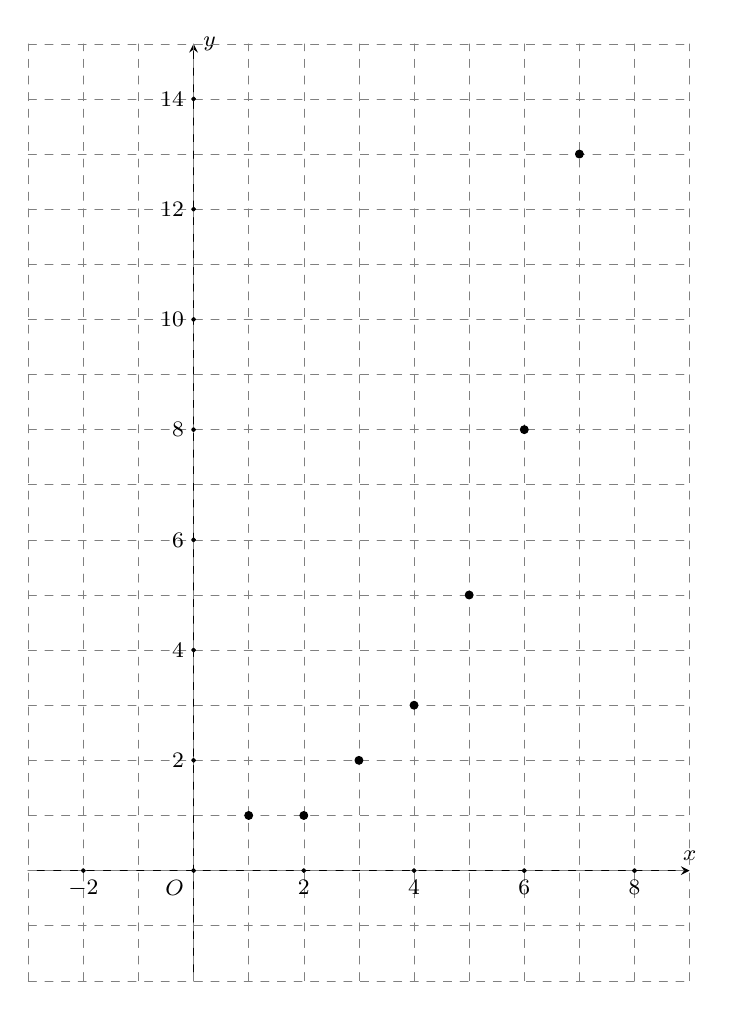
\begin{tikzpicture}[scale=0.7, font=\footnotesize, line join=round, line cap=round, >=stealth]
			\draw[->] (-3,0)--(9,0) node[above]{$x$};
			\draw[->] (0,-2)--(0,15) node[right]{$y$};
			\draw[very thin,step=1cm,color=gray,dashed] (-3,-2)grid(9,15);
			\foreach \i/\j in {1/1,2/1,3/2,4/3,5/5,6/8,7/13}
			\draw[fill=black] (\i,\j)circle(2pt);
			\foreach \i in {-2,2,4,6,8}
			\draw[fill=black] (\i,0)node[below]{$\i$}circle(1pt);
			\foreach \i in {2,4,6,8,10,12,14}
			\draw[fill=black] (0,\i)node[left]{$\i$}circle(1pt);
			\draw[fill=black] (0,0) circle (1pt) node[below left] {$O$};
		\end{tikzpicture}
	\end{center}
}
\end{vd}
\begin{vd}%[0D3H1-4]%[Dự án đề cương 2025]%[Mui Doan]
	Vẽ đồ thị hàm số $f(x)=|x|$, biết rằng hàm số này còn được viết như sau $$f(x)=\heva{&x&\text{với }x\ge 0\\&-x&\text{với }x<0.}$$
	\loigiai{
		Với $x\le 0$ đồ thị hàm số là đường thẳng $y=x$, với $x<0$ đồ thị hàm số là đường thẳng $y=-x$.\\
		Vậy đồ thị hàm số $f(x)=|x|$ có dạng như sau
		\begin{center}
			\begin{tikzpicture}[scale=1, font=\footnotesize, line join=round, line cap=round, >=stealth]
				\draw [->] (-3,0)--(3,0) node[below]{$x$};
				\draw [->] (0,-2)--(0,3) node[right]{$y$};
				\draw[fill=black] (0,0) circle(1pt) node[below left]{$O$};
				\clip (-3,-2) rectangle (3,3);
				\draw[name path=c1,smooth, samples=300, domain=-3:0] plot (\x,{-(\x)});
				\draw[name path=c2,smooth, samples=300, domain=0:3] plot (\x,{(\x)});
				\foreach \i in {-2,-1,1,2} \draw [fill=black] (\i,0) circle(1pt) node[below]{$\i$};
				\foreach \j in {-1,1,2} \draw [fill=black] (0,\j) circle(1pt) node[left]{$\j$};
			\end{tikzpicture}
		\end{center}
	}
\end{vd}
\begin{vd}%[0D3H1-4]%[Dự án đề cương 2025]%[Mui Doan]
	Tìm tập xác định, tập giá trị và vẽ đồ thị hàm số $f(x)=\heva{&-1&\text{với }x<0\\&1&\text{với }x>0.}$
	\loigiai{
		Hàm số có tập xác định là $\mathscr{D}=\mathbb{R}\setminus\{0\}$.\\
		Tập giá trị $T=\{-1;1\}$.\\
		Đồ thị của hàm số
		\begin{center}
			\begin{tikzpicture}[scale=1, font=\footnotesize, line join=round, line cap=round, >=stealth]
				\draw [->] (-3,0)--(3,0) node[below]{$x$};
				\draw [->] (0,-2)--(0,2) node[left]{$y$};
				\draw[fill=black] (0,0) circle(1pt) node[below left]{$O$};
				\clip (-3,-2) rectangle (3,2);
				\draw[name path=c1,smooth, samples=300, domain=-3:0] plot (\x,{-1});
				\draw[name path=c2,smooth, samples=300, domain=0:3] plot (\x,{1});
				\foreach \i in {-2,-1,1,2} \draw [fill=black] (\i,0) circle(1pt) node[below]{$\i$};
				\foreach \j in {1} \draw [fill=black] (0,\j) circle(1pt) node[left]{$\j$};
				\draw[fill=black] (0,-1) circle(1pt) node[right]{$-1$};
			\end{tikzpicture}
		\end{center}
		
	}
\end{vd}
\begin{dang}{Bài toán thực tế liên quan đến hàm số và đồ thị}
	Phương pháp giải
	\begin{itemize}
		\item  Phân tích đề bài: Xác định các đại lượng biến thiên, mối quan hệ giữa chúng và điều kiện ràng buộc.
		\item  Xây dựng công thức hàm số: Dựa trên các thông tin và quy luật đã cho. Thường là hàm từng phần.
		\item  Giải thích đồ thị: Dựa vào hình dạng đồ thị để mô tả sự biến thiên của đại lượng được biểu diễn.
		\item  So sánh, đánh giá: Từ hàm số hoặc đồ thị, đưa ra các nhận định, quyết định.
	\end{itemize}
\end{dang}

\begin{vd}%[0D3H1-7]%[Dự án đề cương 2025]%[Mui Doan]
	Gia đình bạn Sơn sống ở tầng ba, bà ngoại của Sơn sống ở tầng sáu thuộc cùng một chung cư cao tầng. Sơn đi bộ từ nhà mình xuống tầng một để lấy thư và đưa lên nhà bà ngoại. Đưa thư cho bà xong, Sơn quay về nhà mình.\\
	Đặt $y=h(t)$ là hàm số biểu thị khoảng cách từ vị trí của Sơn đến mặt đất theo thời gian $t$ từ khi bạn ấy bắt đầu đi cho đến khi về lại nhà mình (chọn gốc thời gian là lúc Sơn bắt đầu đi lấy thư).\\
	$(C_1)$ hay $(C_2)$ là đồ thị của hàm số $y=h(t)$? Tại sao?
	\begin{center}
		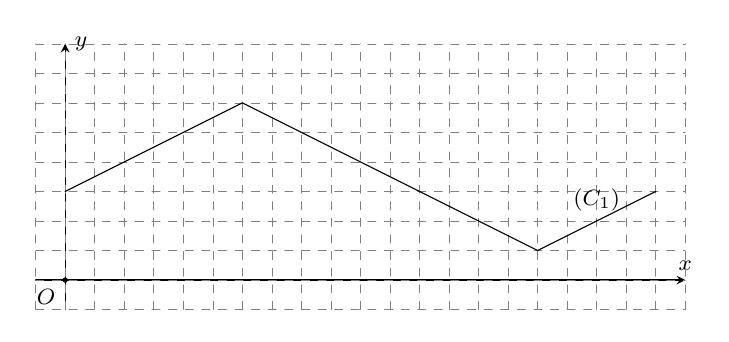
\begin{tikzpicture}[scale=0.75, font=\footnotesize, line join=round, line cap=round, >=stealth]
			\draw[->] (-0.5,0)--(10.5,0) node[above]{$x$};
			\draw[->] (0,-0.5)--(0,4) node[right]{$y$};
			\draw[very thin,step=0.5cm,color=gray,dashed] (-0.5,-0.5)grid(10.5,4);
			\draw (0,1.5)--(3,3)--(8,0.5)--(10,1.5);
			\node[above] at (9,1){$(C_1)$};
			\draw[fill=black] (0,0) circle (1pt) node[below left] {$O$};
		\end{tikzpicture}
		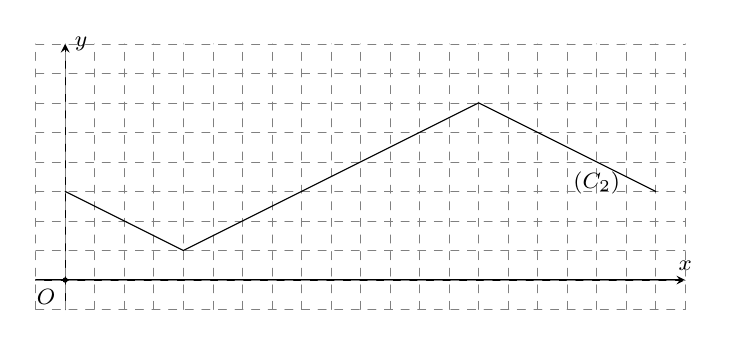
\begin{tikzpicture}[scale=0.75, font=\footnotesize, line join=round, line cap=round, >=stealth]
			\draw[->] (-0.5,0)--(10.5,0) node[above]{$x$};
			\draw[->] (0,-0.5)--(0,4) node[right]{$y$};
			\draw[very thin,step=0.5cm,color=gray,dashed] (-0.5,-0.5)grid(10.5,4);
			\draw (0,1.5)--(2,0.5)--(7,3)--(10,1.5);
			\node[below] at (9,2){$(C_2)$};
			\draw[fill=black] (0,0) circle (1pt) node[below left] {$O$};
		\end{tikzpicture}
	\end{center}
	\loigiai{
		Khi bắt đầu đi từ tầng ba xuống tầng một, Sơn ngày càng gần mặt đất nên khoảng cách từ vị trí của Sơn đến mặt đất giảm dần, hay hàm số giảm, vậy đồ thị phải có dạng đi xuống. \\
		Khi đi từ tầng một lên tầng sáu để đưa thư cho bà ngoại, Sơn ngày càng xa mặt đất nên khoảng cách từ vị trí của Sơn đến mặt đất tăng dần, hay hàm số tăng, vậy đồ thị phải có dạng đi lên.\\
		Khi đi từ tầng sáu về nhà mình, Sơn ngày càng gần mặt đất nên khoảng cách từ vị trí của Sơn đến mặt đất giảm dần, hay hàm số giảm, vậy đồ thị phải có dạng đi xuống.\\
		Đồ thị $(C_2)$ có dạng tương ứng như mô tả ở trên. Do đó, $(C_2)$ là đồ thị của hàm số $y=h(t)$ này.
	}
\end{vd}
\begin{vd}%[0D3V1-7]%[Dự án đề cương 2025]%[Mui Doan]
	Một hãng taxi có bảng giá như sau
	\begin{longtable}{|p{0.15\textwidth}|p{0.25\textwidth}|p{0.25\textwidth}|p{0.25\textwidth}|}
		\hline
		& \textbf{Giá mở cửa ($0{,}5$ km)} & \textbf{Giá cước các kilômét tiếp theo} & \textbf{Giá cước từ kilômét thứ $31$}\\
		\hline 
		Taxi $4$ chỗ & $11000$ đồng & $14500$ đồng & $11600$ đồng\\
		\hline
		Taxi $7$ chỗ & $11000$ đồng & $15500$ đồng & $13600$ đồng\\
		\hline
	\end{longtable}
	\begin{enumerate}[a)]
		\item Xem số tiền đi taxi là một hàm số phụ thuộc số kilômét di chuyển, hãy viết công thức của các hàm số dựa trên thông tin từ bảng giá đã cho theo từng yêu cầu:
		\begin{itemize}
			\item Hàm số $f(x)$ để tính số tiền hành khách phải trả khi di chuyển $x$ km bằng xe taxi $4$ chỗ.
			\item Hàm số $g(x)$ để tính số tiền hành khách phải trả khi di chuyển $x$ km bằng xe taxi $7$ chỗ.
		\end{itemize}
		\item Nếu cần đặt xe taxi cho $30$ hành khách, nên đặt toàn bộ xe $4$ chỗ hay xe $7$ chỗ thì có lợi hơn?
	\end{enumerate}
	\loigiai{
		Gọi $x$ là số kilômét hành khách di chuyển $(x\ge 0)$.
		\begin{enumerate}[a)]
			\item Khi đã lên taxi $4$ chỗ, hành khách luôn phải trả $11000$ đồng dù đi hay không, do đó số tiền phải trả luôn bao gồm $11000$ đồng này.
			\begin{itemize}
				\item Nếu $0\le x\le 0{,}5$ thì số tiền phải trả là $11000$ đồng.
				\item Nếu $0{,}5<x\le 31$ thì số tiền phải trả là 
				$$11000+14500(x-0{,}5)=3750+14500x.$$
				\item Nếu $x>30$ thì số tiền phải trả là
				$$11000+14500\cdot (30-0{,}5)+11600(x-30)=90750+11600x.$$
			\end{itemize}
			Vậy hàm số $f(x)$ có công thức $f(x)=\heva{&11000 &\text{với } 0\le x\le 0{,}5\\&3750+14500x&\text{với } 0{,}5<x\le 30\\&90750+11600x&\text{với } x>30.}$\\
			Tương tự, đối với taxi $7$ chỗ, hàm số $g(x)$ có công thức $g(x)=\heva{&11000 &\text{với } 0\le x\le 0{,}5\\&3250+15500x&\text{với } 0{,}5<x\le 30\\&60250+13600x&\text{với } x>30.}$
			\item Khi có $30$ hành khách, nếu đặt toàn bộ xe $4$ chỗ thì cần đặt $8$ xe. Khi đó, số tiền taxi phải trả là 
			$$f_1(x)=\heva{&8\cdot 11000 &\text{với } 0\le x\le 0{,}5\\&8(3750+14500x)&\text{với } 0{,}5<x\le 30\\&8(90750+11600x)&\text{với } x>30.}$$
			Nếu đặt toàn bộ xe $7$ chỗ thì cần đặt $5$ xe. Khi đó, số tiền taxi phải trả là 
			$$g_1(x)=\heva{&5\cdot 11000 &\text{với } 0\le x\le 0{,}5\\&5(3250+15500x)&\text{với } 0{,}5<x\le 30\\&5(60250+13600x)&\text{với } x>30.}$$
			Ta cần so sánh $f_1(x)$ với $g_1(x)$.\\
			Xét hiệu số $f_1(x)-g_1(x)$.
			\begin{itemize}
				\item Khi $0\le x\le 0{,}5$, ta có
				$f_1(x)-g_1(x)=8\cdot 11000-5\cdot 11000=33000>0$.\\
				Do đó $f_1(x)>g_1(x)$.\\
				Nghĩa là khi $30$ người di chuyển quãng đường ít hơn hoặc bằng $0{,}5$ km bằng taxi thì đi xe $4$ chỗ sẽ tốn nhiều tiền hơn đi xe $7$ chỗ.
				\item Khi $0{,}5<x\le 30$, ta có
				$$f_1(x)-g_1(x)=8(3750+14500x)-5(3250+15500x)=13750+38500x.$$
				Vì $x>0$ nên $f_1(x)-g_1(x)>0$ hay $f_1(x)>g_1(x)$.\\
				Nghĩa là khi $30$ người di chuyển quãng đường trên $0{,}5$ km đến $30$ km bằng taxi thì đi xe $4$ chỗ sẽ tốn nhiều tiền hơn đi xe $7$ chỗ.
				\item Khi $x>30$, ta có 
				$$f_1(x)-g_1(x)=8(90750+11600x)-5(60250+13600x)=424750+24800x.$$
				Vì $x>0$ nên $f_1(x)-g_1(x)>0$ hay $f_1(x)>g_1(x)$.\\
				Nghĩa là khi $30$ người di chuyển quãng đường từ $30$ km trở đi bằng taxi thì đi xe $4$ chỗ sẽ tốn nhiều tiền hơn đi xe $7$ chỗ.
			\end{itemize}
			Từ ba trường hợp trên, ta đưa ra kết luận: Nếu cần đặt xe taxi cho $30$ hành khách thì nên đặt toàn bộ xe $7$ chỗ sẽ có lợi hơn (tiết kiệm chi phí hơn đặt toàn bộ xe $4$ chỗ).
		\end{enumerate}
	}
\end{vd}

%-----------------------------------------------------------------------------
\subsection{Bài tập rèn luyện}
\ind{PHẦN I.} \inden{Câu trắc nghiệm nhiều phương án lựa chọn. Mỗi câu hỏi học sinh chỉ chọn một phương án.}\\
\setcounter{ex}{0}
\Opensolutionfile{ans}[ans/0D3-Bai1-TN]%--Đặt tên 2D1-Bai1-Dang1-TN
\begin{ex}%[0D3N1-1]
	[Trích đề thi giữa kỳ I lớp 10 -THPT Tân Túc -TP HCM-Năm học 2023-2024]
	Tập xác định của hàm số $y=f(x)=\sqrt{x-1}$ là
	\choice
	{$\mathscr{D}=(1;+\infty)$}
	{$\mathscr{D}=\mathbb{R} \backslash\{1\}$}
	{\True $\mathscr{D}=[1;+\infty)$}
	{$\mathscr{D}=\mathbb{R}$}
	\loigiai{
		Điều kiện $x-1\geq0\Leftrightarrow x\geq1$.\\
		Vậy $\mathscr{D}=[1;+\infty)$.
	}
\end{ex}

\begin{ex}%[0D3N1-2]
	[Trích đề thi giữa kỳ II lớp 10 -THPT Chuyên Hùng Vương-Phú Thọ-Năm học 2023-2024]
	Cho hàm số $y=f(x)$ có đồ thị như hình vẽ sau
	\begin{center}
		\begin{tikzpicture}[scale=1, font=\footnotesize, line join=round, line cap=round, >=stealth]
			\def\xmin{-3.5}\def\xmax{3.5}\def\ymin{-1.5}\def\ymax{4.5}
			\draw[->] (\xmin-0.2,0)--(\xmax+0.2,0) node[below] {\footnotesize $x$};
			\draw[->] (0,\ymin-0.2)--(0,\ymax+0.2) node[right] {$y$};
			\draw (0,0) node [below left] {$O$};
			\foreach \x in {-1,1,3}\draw (\x,0.05)--(\x,-0.05) node [below] {\footnotesize $\x$};
			\foreach \x in {-3}\draw (\x,0.05)--(\x,-0.05) node [above] {\footnotesize $\x$};
			\foreach \y in {-1,1}\draw (0.05,\y)--(-0.05,\y) node [right] {\footnotesize $\y$};
			\foreach \y in {4}\draw (0.05,\y)--(-0.05,\y) node [left] {\footnotesize $\y$};
			\clip (\xmin,\ymin) rectangle (\xmax,\ymax);
			\coordinate (A) at (-3,-1);
			\coordinate (B) at (-1,1);
			\coordinate (C) at (1,0);
			\coordinate (D) at (3,4);
			\draw (A)--(B)--(C)--(D);
			\draw [dashed] (-3,0)--(A)--(0,-1) (-1,0)--(B)--(0,1) (0,4)--(D)--(3,0);
			\foreach \diem in {A,B,C,D}	\fill (\diem)circle(1pt);
		\end{tikzpicture}
	\end{center}
	Tập xác định của hàm số $y=f(x)$ là
	\choice
	{\True $\mathscr{D}=[-3;3]$}
	{$\mathscr{D}=[-1;4]$}
	{$\mathscr{D}=[-3;4]$}
	{$\mathscr{D}=\mathbb{R}$}
	\loigiai{
		Dựa vào đồ thị hàm số ta thấy tập xác định của hàm số là $\mathscr{D}=[-3;3]$.
	}
\end{ex}

\begin{ex}%[0D3H1-2]
	[Trích đề thi giữa kỳ I lớp 10 -THPT Hoàng Hoa Thám - Tp HCM-Năm học 2023-2024]
	Tập xác định của hàm số $f(x)=\dfrac{x+5}{x-1}+\dfrac{x-1}{x+5}$ là
	\choice
	{$\mathscr{D}=\mathbb{R}\setminus \{1\}$}{\True $\mathscr{D}=\mathbb{R}\setminus\{-5;1\}$}
	{$\mathscr{D}=\mathbb{R}\setminus\{-5\}$}
	{$\mathscr{D}=\mathbb{R}$
	}
	\loigiai{
		Hàm số xác định khi và chỉ khi
		$\heva{&x-1\neq0\\ &x+5\neq 0}\Leftrightarrow\heva{&x\neq 1\\ &x\neq -5.}$\\
		Vậy tập xác định của hàm số là $\mathscr{D}=\mathbb{R}\setminus\{-5;1\}$.
	}
\end{ex}


\begin{ex}%[0D3H1-4]%[Dự án đề cương 2025]%[Mui Doan]
Cho hàm số $y=f(x)=\dfrac{1}{8} x^{2}$ xác định trên $\mathscr{D}=[-3 ; 5]$. Điểm nào sau đây thuộc đồ thị của hàm số?
\choice
{$A(8;1)$}
{$B(-4;2)$}
{\True $C(4;2)$}
{$D(0;1)$}
\loigiai{
	Để một điểm thuộc đồ thị hàm số, tọa độ của điểm đó phải thỏa mãn phương trình hàm số và hoành độ thuộc tập xác định.\\
	Với $C(4;2)$: $x=4 \in [-3;5]$. Thay $x=4$ vào hàm số, ta có $y=\dfrac{1}{8} \cdot 4^2 = \dfrac{1}{8} \cdot 16 = 2$.\\
	Vậy điểm $C(4;2)$ thuộc đồ thị hàm số. 
}
\end{ex}

\begin{ex}%[0D3N1-5]%[Dự án đề cương 2025]%[Mui Doan]
Hàm số $y=3x-1$ là hàm số
\choice
{Nghịch biến trên $\mathbb{R}$}
{Đồng biến trên $(-\infty;0)$ và nghịch biến trên $(0;+\infty)$}
{\True Đồng biến trên $\mathbb{R}$}
{Không đồng biến cũng không nghịch biến}
\loigiai{
	Với hàm số $y=f(x)=3x-1$, ta có hệ số $a=3> 0$.
	Do đó, hàm số đồng biến trên $\mathbb{R}$. 
}
\end{ex}

\begin{ex}%[0D3N1-5]%[Dự án đề cương 2025]%[Mui Doan]
Hàm số $f(x)=-5x+2$ là hàm số
\choice
{\True Nghịch biến trên $\mathbb{R}$}
{Đồng biến trên $\mathbb{R}$}
{Đồng biến trên $(-\infty;0)$ và nghịch biến trên $(0;+\infty)$}
{Không đồng biến cũng không nghịch biến}
\loigiai{
	Với hàm số $f(x)=-5x+2$, ta có hệ số $a=-5 < 0$.
	Do đó, hàm số nghịch biến trên $\mathbb{R}$. 
}
\end{ex}

\begin{ex}%[0D3N1-5]%[Dự án đề cương 2025]%[Mui Doan]
	Quan sát đồ thị hàm số sau
	\begin{center}
		\begin{tikzpicture}[scale=0.6, font=\footnotesize, line join=round, line cap=round, >=stealth]
			\draw[->] (-5,0)--(9,0) node[above]{$x$};
			\draw[->] (0,-3)--(0,5) node[right]{$y$};
			\draw[very thin,step=1cm,color=gray,dashed] (-5,-3)grid(9,5);
			\draw (-3,-2)--(-2,2)--(5,1.2)--(7,3);
			\foreach \i/\j in {-3/-2,7/3}
			\draw[fill=black] (\i,\j)circle(2pt);
			\foreach \i in {-4,-2,2,4,6,8}
			\draw[fill=black] (\i,0)node[below]{$\i$}circle(1pt);
			\foreach \i in {-2,2,4}
			\draw[fill=black] (0,\i)node[above right=-0.15 and 0]{$\i$}circle(1pt);
			\draw[fill=black] (0,0) circle (1pt) node[below left] {$O$};
		\end{tikzpicture}
	\end{center}
	\choice
	{Đồng biến}
	{\True Nghịch biến}
	{Không đổi}
	{Không xác định}
\loigiai{
	Trên khoảng $(-2;5)$, đồ thị có dạng đi xuống từ trái sang phải nên hàm số này nghịch biến trên khoảng $(-2;5)$.
}
\end{ex}

\begin{ex}%[0D3H1-2]
	[Trích đề thi giữa kỳ 2 lớp 10-THPT Lương Ngọc Quyến - Thái Nguyên-Năm học 2023-2024]
	Xét hàm số $y=f(x)$ cho bởi bảng sau\begin{center}
		\begin{tabular}{|c|c|c|c|c|c|c|c|c|}
			\hline
			$x$ & $1$ & $4$ & $7$ & $10$ & $13$ & $16$ & $19$ & $22$ \\
			\hline
			$y$ & $28$ & $27$ & $28$ & $32$ & $31$ & $29$ & $28$ & $27$ \\
			\hline
		\end{tabular}
	\end{center}
	Tập xác định của hàm số có số phần tử là
	\choice
	{\True $8$}
	{$22$}
	{$10$}
	{$5$}
	\loigiai{Tập xác định của hàm số $y=f(x)$ là $\left\{1;4;7;10;13;16;19;22\right\}$. Do đó số phần tử của tập xác định này là $8$.}
\end{ex}

\begin{ex}%[0D3H1-2]%[Dự án đề cương 2025]%[Mui Doan]
Tìm tập xác định của hàm số $f(x)=2+\dfrac{1}{x+3}$.
\choice
{\True $\mathscr{D}=\mathbb{R}\setminus {-3}$}
{$\mathscr{D}=\mathbb{R}$}
{$\mathscr{D}=(-\infty;-3]$}
{$\mathscr{D}=(-3;+\infty)$}
\loigiai{
	Hàm số xác định khi và chỉ khi mẫu số $x+3\ne 0$, tức là $x\ne -3$.\\
	Vậy tập xác định $\mathscr{D}=\mathbb{R}\setminus {-3}$.
}
\end{ex}

\begin{ex}%[0D3H1-5]%[Dự án đề cương 2025]%[Mui Doan]
Xét hàm số $y=x^{2}$ trên khoảng $(-\infty;0)$. Kết luận nào sau đây là đúng?
\choice
{Hàm số đồng biến trên khoảng $(-\infty;0)$}
{\True Hàm số nghịch biến trên khoảng $(-\infty;0)$}
{Hàm số không đồng biến cũng không nghịch biến trên khoảng $(-\infty;0)$}
{Không thể xác định}
\loigiai{
	Lấy $x_1$, $x_2$ tuỳ ý sao cho $x_1<x_2$ và $x_1, x_2 \in(-\infty;0)$.\\
	Ta có $f(x_1)-f(x_2)=x_1^2-x_2^2=(x_1-x_2)(x_1+x_2)$.\\
	Do $x_1<x_2$ nên $x_1-x_2<0$.\\
	Do $x_1$, $x_2 \in(-\infty;0)$ nên $x_1<0$ và $x_2<0$, suy ra $x_1+x_2<0$.\\
	Vậy $f(x_1)-f(x_2) = (x_1-x_2)(x_1+x_2) > 0$.\\
	Nghĩa là $f(x_1)>f(x_2)$.\\
	Vậy hàm số nghịch biến trên khoảng $(-\infty;0)$.
}
\end{ex}

\begin{ex}%[0D3H1-7]%[Dự án đề cương 2025]%[Mui Doan]
Một hãng taxi có giá mở cửa là $11\,000$ đồng cho $0{,}5$ km đầu tiên và $14\,500$ đồng cho mỗi kilômét tiếp theo (đến $30$ km). Nếu khách đi $2$ km bằng xe taxi $4$ chỗ thì số tiền phải trả là bao nhiêu?
\choice
{$11\,000$ đồng}
{$14\,500$ đồng}
{\True $32\,750$ đồng}
{$29\,000$ đồng}
\loigiai{
	Gọi $x$ là số kilômét di chuyển.\\
	Nếu $0{,}5< x \le 30$, công thức tính tiền là $11\,000 + 14\,500(x-0{,}5) = 3\,750 + 14\,500x$.\\
	Với $x=2$ km: $2> 0{,}5$, nên áp dụng công thức trên.\\
	Số tiền phải trả là $3\,750 + 14\,500 \cdot 2 =32\,750$ đồng. 
}
\end{ex}

\begin{ex}%[0D3H1-4]%[Dự án đề cương 2025]%[Mui Doan]
Biểu thức $f(x)$ mô tả sự biến đổi của số $x$ trong \lq\lq Hộp đen\rq\rq\, qua các máy: \lq\lq Máy bình phương\rq\rq $\rightarrow$ \lq\lq Máy tăng gấp ba lần\rq\rq $\rightarrow$ \lq\lq Máy lấy bớt đi $5$\rq\rq\, là
\begin{center}
	\begin{tikzpicture}[scale=1, font=\footnotesize, line join=round, line cap=round, >=stealth]
		\tikzstyle{hop1}=[
		minimum height=1.2cm,
		minimum width=4cm,
		align=center,
		anchor=center,
		rounded corners=4pt,
		drop shadow=gray]
		\tikzstyle{hop2}=[
		below,
		minimum height=1cm,
		minimum width=4cm,
		align=center,
		anchor=center,
		rounded corners=4pt,
		drop shadow=gray]
		\mathversion{bold}
		\path (0,0) node[hop1,fill=orange!50] (a){$x$};
		\path(a.east)--+(4,0) node[hop1,fill=black] (b){\textbf{HỘP ĐEN HỘP ĐEN HỘP ĐEN}\\ \textbf{HỘP ĐEN HỘP ĐEN HỘP ĐEN}\\ \textbf{HỘP ĐEN HỘP ĐEN HỘP ĐEN}};
		\path(b.east)--+(3,0) node[hop2,fill=blue!50] (c){\color{white}{$f(x)$?}};
		\draw[thick,->] (a)--(b);
		\draw[thick,->] (b)--(c);
		\path (b.center) --+(0,-1.3) node{\bf Điều gì đã xảy ra bên trong HỘP ĐEN?};
	\end{tikzpicture}
\end{center}
\choice
{$f(x) = (3x)^2 - 5$}
{$f(x) = x^2 - 5\cdot3$}
{$f(x) = 3(x-5)^2$}
{\True $f(x) = 3x^2 - 5$}
\loigiai{
	Số $x$ đi qua \lq\lq máy bình phương\rq\rq\, thì biến đổi thành $x^2$.\\
	$x^2$ đi qua \lq\lq máy tăng gấp ba lần\rq\rq\, thì biến đổi thành $3x^2$.\\
	$3x^2$ đi qua \lq\lq qmáy lấy bớt đi $5$ \lq\lq\, thì biến đổi thành $3x^2-5$.\\
	Vậy $f(x)=3x^2-5$. 
}
\end{ex}

\begin{ex}%[0D3N1-5]
	[Trích đề thi giữa kỳ 2 lớp 10-THPT Nguyen Thái Bình-Năm học-2024-2025]
	Cho hàm số $y=f(x)$ có bảng biến thiên như hình bên dưới. Khẳng định nào sao đây là đúng?
	\begin{center}
		
\begin{tikzpicture}
			\tkzTabInit[espcl=2.5,lgt=1.5]
			{$x$/0.7,$y$/2.1}
			{$-\infty$,$0$,$+\infty$}
			%\tkzTabLine{,+,0,-,}
			\tkzTabVar{-/$-\infty$,+/$1$,-/$-\infty$}
		\end{tikzpicture}
	\end{center}
	\choice
	{Hàm số đồng biến trên khoảng $(-\infty;1)$}
	{Hàm số đồng biến trên khoảng $(1;+\infty)$}
	{Hàm số đồng biến trên khoảng $(-\infty;+\infty)$}
	{\True Hàm số đồng biến trên khoảng $(-\infty;0)$}
	\loigiai{
		Từ bảng biến thiên ta thấy hàm số đồng biến trên khoảng $(-\infty;0)$.
	}
\end{ex}

\begin{ex}%[0D3H1-4]%[Dự án đề cương 2025]%[Mui Doan]
Hàm số $f(x)$ được cho bởi bảng sau:
\begin{center}
\begin{tabular}{|c|c|c|c|c|c|c|c|}
	\hline
	$x$ & $1$ & $2$ & $3$ & $4$ & $5$ & $6$ & $7$ \\
	\hline
	$f(x)$ & $1$ & $1$ & $2$ & $3$ & $5$ & $8$ & $13$ \\
\hline
\end{tabular}
\end{center}
Điểm nào sau đây thuộc đồ thị của hàm số?
\choice
{$(0;0)$}
{$(2;3)$}
{\True $(4;3)$}
{$(7;8)$}
\loigiai{
	Dựa vào bảng giá trị, ta tìm cặp $(x;f(x))$ phù hợp.
	Kiểm tra các đáp án
	\begin{itemize}
		\item $(0;0)$: Không có trong bảng.
		\item $(2;3)$: Khi $x=2$, $f(x)=1$, không phải $3$.
		\item $(4;3)$: Khi $x=4$, $f(x)=3$. Đây là điểm thuộc đồ thị.
		\item $(7;8)$: Khi $x=7$, $f(x)=13$, không phải $8$.
	\end{itemize}
	Vậy điểm $(4;3)$ thuộc đồ thị hàm số. 
}
\end{ex}
\begin{ex}%[0D3N1-3]
	[10 HK1 NH24-25-THPT Mạc Đĩnh Chi - TP.HCM]
	Cho hàm số $f(x)=\heva{&x+1 &\text{khi } x\ge 3\\&10-2x &\text{khi } x < 3}$. Tính $f(4)$ .
	\choice
	{\True $5$}
	{$2$}
	{$3$}
	{$18$}
	\loigiai{
		Ta có $ 4 \ge 3 $ nên $ f(4)=4+1=5 $.
	}
\end{ex}

\begin{ex}%[0D3H1-3]%[Dự án đề cương 2025]%[Mui Doan]
Cho hàm số $f(x)=\heva{&-1&\text{với }x<0\\&1&\text{với }x>0.}$\\
Tập giá trị của hàm số là
\choice
{$\mathbb{R}$}
{$\{-1\}$}
{$\{1\}$}
{\True $\{-1;1\}$}
\loigiai{
	Hàm số này chỉ nhận hai giá trị là $-1$ (khi $x<0$) và $1$ (khi $x>0$).
	Do đó, tập giá trị của hàm số là $T=\{-1;1\}$.
}
\end{ex}

\begin{ex}%[0D3H1-5]%[Dự án đề cương 2025]%[Mui Doan]
Hàm số nào sau đây là hàm số đồng biến trên $\mathbb{R}$?
\choice
{$y = -2x+1$}
{$y = x^2$}
{\True $y = \dfrac{1}{2}x - 5$}
{$y = -x^3$}
\loigiai{
	Hàm số bậc nhất $y=ax+b$ đồng biến khi $a>0$.
	\begin{itemize}
		\item $y=-2x+1$: có $a=-2<0$, nghịch biến.
		\item $y=x^2$: đồng biến trên $(0;+\infty)$ và nghịch biến trên $(-\infty;0)$, không đồng biến trên $\mathbb{R}$.
		\item $y=\dfrac{1}{2}x-5$: có $a=\dfrac{1}{2}>0$, đồng biến trên $\mathbb{R}$.
		\item $y=-x^3$: nghịch biến trên $\mathbb{R}$.
	\end{itemize}
	Vậy hàm số $y=\dfrac{1}{2}x-5$ là hàm số đồng biến trên $\mathbb{R}$. 
}
\end{ex}

\begin{ex}%[0D3H1-5]%[Dự án đề cương 2025]%[Mui Doan]
Hàm số nào sau đây là hàm số nghịch biến trên $\mathbb{R}$?
\choice
{$y=2x-3$}
{$y=x+5$}
{\True $y=-3x+7$}
{$y=x^2+1$}
\loigiai{
	Hàm số bậc nhất $y=ax+b$ nghịch biến khi $a<0$.
	\begin{itemize}
		\item $y=2x-3$: có $a=2>0$, đồng biến.
		\item $y=x+5$: có $a=1>0$, đồng biến.
		\item $y=-3x+7$: có $a=-3<0$, nghịch biến trên $\mathbb{R}$.
		\item $y=x^2+1$: đồng biến trên $(0;+\infty)$ và nghịch biến trên $(-\infty;0)$, không nghịch biến trên $\mathbb{R}$.
	\end{itemize}
Vậy hàm số $y=-3x+7$ là hàm số nghịch biến trên $\mathbb{R}$. 
}
\end{ex}

\begin{ex}%[0D3H1-3]%[Dự án đề cương 2025]%[Mui Doan]
Cho hàm số $f(x)=x^2+3$. Giá trị $f(-2)$ là:
\choice
{$-1$}
{$1$}
{$4$}
{\True $7$}
\loigiai{
	Thay $x=-2$ vào công thức hàm số:
	$f(-2) = (-2)^2 + 3 = 4 + 3 = 7$.
}
\end{ex}

\begin{ex}%[0D3H1-3]%[Dự án đề cương 2025]%[Mui Doan]
Cho hàm số $f(x)$ được cho bởi bảng sau:
\begin{center}
\begin{tabular}{|c|c|c|c|c|}
	\hline
	$x$ & $-1$ & $0$ & $1$ & $2$ \\
	\hline
	$f(x)$ & $5$ & $3$ & $1$ & $-1$ \\
	\hline
\end{tabular}
\end{center}
Giá trị của $f(0)$ là:
\choice
{$-1$}
{$1$}
{\True $3$}
{$5$}
\loigiai{
	Dựa vào bảng giá trị, khi $x=0$, ta có $f(x)=3$.
	Vậy $f(0)=3$.
}
\end{ex}

\begin{ex}%[0D3H1-4]%[Dự án đề cương 2025]%[Mui Doan]
Trong các hàm số sau, hàm số nào có đồ thị là đường thẳng?
\choice
{$y=x^2-1$}
{$y=\sqrt{x}$}
{\True $y=2x+3$}
{$y=\dfrac{1}{x}$}
\loigiai{
	Đồ thị của hàm số bậc nhất $y=ax+b$ ($a \ne 0$) là một đường thẳng.
	\begin{itemize}
		\item $y=x^2-1$: là hàm số bậc hai, đồ thị là parabol.
		\item $y=\sqrt{x}$: là hàm số chứa căn, đồ thị là một nửa parabol.
		\item $y=2x+3$: là hàm số bậc nhất với $a=2, b=3$, đồ thị là đường thẳng.
		\item $y=\dfrac{1}{x}$: là hàm số phân thức, đồ thị là hypebol.
	\end{itemize}
	Vậy $y=2x+3$ có đồ thị là đường thẳng.
}
\end{ex}

\begin{ex}%[0D3H1-4]%[Dự án đề cương 2025]%[Mui Doan]
Điểm nào sau đây là giao điểm của đồ thị hàm số $y=2x-4$ với trục hoành?
\choice
{$(0;4)$}
{$(0;-4)$}
{\True $(2;0)$}
{$(-2;0)$}
\loigiai{
	Giao điểm với trục hoành là điểm có tung độ $y=0$.
	Thay $y=0$ vào phương trình hàm số: $0 = 2x-4 \Rightarrow 2x=4 \Rightarrow x=2$.
	Vậy giao điểm là $(2;0)$.
}
\end{ex}

\begin{ex}%[0D3H1-4]%[Dự án đề cương 2025]%[Mui Doan]
Điểm nào sau đây là giao điểm của đồ thị hàm số $y=-x+5$ với trục tung?
\choice
{$(5;0)$}
{\True $(0;5)$}
{$(-5;0)$}
{$(0;-5)$}
\loigiai{
	Giao điểm với trục tung là điểm có hoành độ $x=0$.\\
	Thay $x=0$ vào phương trình hàm số: $y = -0+5 \Rightarrow y=5$.\\
	Vậy giao điểm là $(0;5)$.
}
\end{ex}
\begin{ex}%[0D3H1-2]
	[10 học kì 1 NH24-25-THPT Nguyễn Thị Minh Khai  - TpHCM]
	Tìm tập xác định $\mathscr{D}$ của hàm số $f(x)=\sqrt{x}+\dfrac{1}{x-1}$.
	\choice
	{$\mathscr{D}=\mathbb{R} \setminus\{1\}$}
	{$\mathscr{D}=[0;+\infty)$}
	{\True $\mathscr{D}=[0; 1) \cup(1;+\infty)$}
	{$\mathscr{D}=(0;+\infty) \setminus\{1\}$}
	\loigiai{
		Biểu thức $\sqrt{x}+\dfrac{1}{x-1}$ có nghĩa khi $\heva{&x\geq 0\\&x-1\ne 0} \Rightarrow \heva{&x\geq 0\\&x\ne1.}$\\
		Vậy tập xác định hàm số $f(x)=\sqrt{x}+\dfrac{1}{x-1}$ là $\mathscr{D}=[0; 1) \cup(1;+\infty)$.
	}
\end{ex}

\Closesolutionfile{ans}

\ind{PHẦN II.} \inden{Câu trắc nghiệm đúng sai. Trong mỗi ý a), b), c), d) ở mỗi câu, học sinh chọn đúng hoặc sai.}\\
\setcounter{ex}{0}
\Opensolutionfile{ans}[ans/0D3-Bai1-DS]%--Đặt tên 2D1-Bai1-DS
\begin{ex}%[0D3H1-5]%[Dự án đề cương 2025]%[Mui Doan]
	Cho hàm số $y=ax+b$ có đồ thị đi qua điểm $A(1;5)$ và $B(-1;1)$. 
	\choiceTF
	{\True Giá trị của $a$ là $2$}
	{Giá trị của $b$ là $4$}
	{\True Phương trình hàm số là $y=2x+3$}
	{Hàm số nghịch biến trên $\mathbb{R}$}
	\loigiai{
		Đồ thị hàm số đi qua $A(1;5)$ và $B(-1;1)$, ta có hệ phương trình
		$\heva{&a\cdot )+b=5 \\ &a\cdot (-1)+b=1} \Leftrightarrow \heva{&a+b=5 \\ &-a+b=1}\Leftrightarrow\heva{&a=2\\&b=3.}$
		\begin{itemchoice}
			\itemch Ta có $a=2$.
			\itemch Ta có $b=3$.
			\itemch  Phương trình hàm số là $y=2x+3$.
			\itemch Vì $a=2>0$, hàm số đồng biến trên $\mathbb{R}$.
		\end{itemchoice}
	}
\end{ex}
\begin{ex}%[0D3H1-5]%[Dự án đề cương 2025]%[Mui Doan]
	Cho hàm số $f(x) =\heva{&x+2 & \text{khi } x \le 0 \\& 3x+2 & \text{khi } x > 0.}$ 
	\choiceTF
	{\True Giá trị $f(-1)$ là $1$}
	{Giá trị $f(1)$ là $3$}
	{\True Giá trị $f(0)$ là $x=2$}
	{\True Hàm số đồng biến trên từng khoảng xác định}
	\loigiai{
		\begin{itemchoice}
			\itemch Với $x=-1 \le 0$, ta dùng công thức $f(x)=x+2$. Ta có $f(-1) = -1+2=1$.
			\itemch Với $x=1 > 0$, ta dùng công thức $f(x)=3x+2$. Ta có $f(1) = 3(1)+2=5$. 
			\itemch $f(0) = 0+2 = 2$.
			\itemch 
			\begin{itemize}
				\item Trên $(-\infty;0]$: $f(x)=x+2$ có hệ số $a=1>0$, nên đồng biến.
				\item Trên $(0;+\infty)$: $f(x)=3x+2$ có hệ số $a=3>0$, nên đồng biến.
			\end{itemize}
		Do đó hàm số đồng biến trên từng khoảng xác định.
		\end{itemchoice}
	}
\end{ex}

\begin{ex}%[0D3H1-2]%[Dự án đề cương 2025]%[Mui Doan]
	Cho hàm số $f(x) = \sqrt{3-x} + \dfrac{1}{x-1}$. 
	\choiceTF
	{\True Tập xác định của hàm số là $\mathscr{D}=(-\infty;3]\setminus\{1\}$}
	{Hàm số xác định với mọi $x \le 3$}
	{Giá trị $f(2)$ bằng $1$}
	{Hàm số không xác định tại $x=1$ và $x=3$}
	\loigiai{
		Điều kiện $\heva{&3-x \ge 0\\&x-1 \ne 0} \Leftrightarrow \heva{&x \le 3\\&x \ne 1.}$
		\begin{itemchoice}
			\itemch Tập xác định của hàm số là $\mathscr{D}=(-\infty;3]\setminus\{1\}$.
			\itemch Sai vì tại $x=1$ hàm số không xác định.
			\itemch Ta có $2\in\mathscr{D}$, $f(2) = \sqrt{3-2} + \dfrac{1}{2-1}=2$. 
			\itemch Hàm số không xác định tại $x=1$, nhưng xác định tại $x=3$ và  $f(3)=\sqrt{3-3}+\dfrac{1}{3-1}=\dfrac{1}{2}$.
		\end{itemchoice}
	}
\end{ex}
\begin{ex}%[0D3V1-7]
	[Trích đề thi học kỳ 1 lớp 10-THPT Chuyên Lê Quý Đôn - Ninh Thuận]
	Thành phố Hồ Chí Minh ghi nhận số ca mắc mới Covid-$19$ trong các tuần đầu năm $2023$ như biểu đồ dưới đây.
	\begin{center}
		\begin{tikzpicture}[scale=0.6, font=\footnotesize, line join=round,
			line cap=round, >=stealth]
			\node at (8, -1.5)  {Tuần năm 2023};
			\node[rotate=90] at (-1.75, 10)  {Số ca mới mắc};
			\node[align=center] at (8, 13)  {Diễn tiến ca bệnh COVID-19 theo tuần năm 2023 \\ tại thành phố Hồ Chí Minh};
			\begin{scope}
				\clip (-2,-1.5) rectangle (16,12);
				\draw[dashed,gray!50!white,xstep=16.3, ystep=1] (0,0) grid (16,11);
				\path (0,0) node[left] {0};
				\foreach \x in {5,10,15,20,25,30,35,40,45,50}{
					\pgfmathsetmacro{\tungdo}{\x/5}
					\path (0,\tungdo) node[left] {\x};}
				\foreach \x/\y in {1/1,2/2,3/3,4/4,5/5,6/6,7/7,8/8,9/9,10/10,11/11,12/12,13/13,14/14,15/15}{
					\path (\y,0) node [below]{\x};}
				\foreach \x/\y in
				{1/47,2/28,3/16,4/6,5/8,6/6,7/6,8/3,9/4,10/3,11/5,12/6,13/4,14/6,15/33}
				{
					\pgfmathsetmacro{\tungdo}{\y/5}
					\draw[fill=orange!20!white](\x+.25,0) rectangle (\x-.25,\tungdo);
					\path (\x,\tungdo) node [blue,above]{\bfseries \y};}
			\end{scope}
			\draw[->](0,0)--(0,11);
			\draw[->](0,0)--(16,0);
			;
		\end{tikzpicture}
	\end{center}
	Đặt $y$ là số ca mắc mới Covid-19 tương ứng với với tuần thứ $x$ thì phép đặt đó cho ta một hàm số $y=f(x)$.
	\choiceTF
	{\True $f(3)=16$}
	{Tập giá trị của hàm số là $T=[0;50]$}
	{\True Trong $4$ tuần đầu năm 2023, hàm số $y=f(x)$ nghịch biến}
	{Giá trị lớn nhất, giá trị nhỏ nhất của hàm số $y=f(x)$ lần lượt là $M$, $m$. Khi đó $M-m=14$}
	\loigiai{
		\begin{itemchoice}
			\itemch  Với $x=3$ thì số ca mắc bệnh là $16$.
			\itemch  Tập giá trị của hàm số là $T=[3;47]$.
			\itemch  Trong $4$ tuần đầu năm 2023, hàm số $y=f(x)$ nghịch biến.
			\itemch  Giá trị lớn nhất, giá trị nhỏ nhất của hàm số $y=f(x)$ lần lượt là $M=47$, $m=3$. Khi đó $M-m=47-3=44$.
		\end{itemchoice}
	}
\end{ex}

\begin{ex}%[0D3V1-7]%[Dự án đề cương 2025]%[Mui Doan]
	Một hãng xe đạp điện đưa ra bảng giá cho thuê xe như sau $50\,000$ đồng cho giờ đầu tiên, và $30\,000$ đồng cho mỗi giờ tiếp theo (tính theo từng giờ, không làm tròn). Gọi $T(x)$ là tổng số tiền thuê xe trong $x$ giờ ($x$ là số nguyên dương).
	\choiceTF
	{\True Nếu thuê xe $3$ giờ, số tiền phải trả là $110\,000$ đồng}
	{Công thức biểu diễn số tiền thuê xe là $T(x) = 50\,000 + 30\,000x$}
	{\True Nếu thuê xe $0{,}5$ giờ, số tiền phải trả là $50\,000$ đồng}
	{Hàm số $T(x)$ là hàm số nghịch biến}
	\loigiai{
		Công thức của hàm số $T(x)$ (với $x$ là số giờ nguyên dương)
		$T(x)=\heva{&50\,000&~\text{nếu}~&x=1\\&50\,000 + 30\,000(x-1)&~\text{nếu}~ &x>1.}$
		\begin{itemchoice}
			\itemch Với $x=3$, $T(3) = 50\,000 + 30\,000\cdot (3-1)=110\,000$ đồng.
			\itemch Ta có $T(x)=\heva{&50\,000&~\text{nếu}~&x=1\\&50\,000 + 30\,000(x-1)&~\text{nếu}~ &x>1.}$
			\itemch Vì giá thuê tính theo giờ (và $0{,}5$ giờ sẽ được tính là $1$ giờ đầu tiên), nên số tiền phải trả là $50\,000$ đồng.
			\itemch Vì giá thuê xe tăng lên theo số giờ thuê, hàm số $T(x)$ là hàm đồng biến.
		\end{itemchoice}
	}
\end{ex}
\begin{ex}%[0D3H1-5]
	[10 GHKI NH24-25-THPT Nguyễn Thị Minh Khai - Tp.HCM]
	Cho hàm số $f(x) = |x - 4|$.
	\choiceTF
	{\True Tập xác định của hàm số đã cho là $\mathscr{D} = \mathbb{R}$}
	{$f(x) = \heva{&x - 4 &\textrm{ khi $x < 4$}\\&-x + 4 &\textrm{ khi $x \geq 4$}}$}
	{Hàm số đã cho nghịch biến trên khoảng $(4;+\infty)$ và đồng biến trên khoảng $(-\infty;4)$}
	{\True Đồ thị của hàm số đã cho là \\
		\centerline{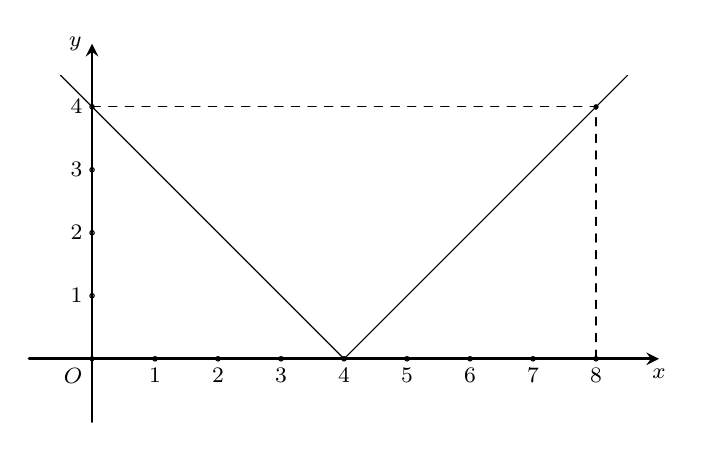
\begin{tikzpicture}[>=stealth,line join=round,line cap=round,font=\footnotesize,scale=0.8]
				\draw[->,line width = 1pt] (-1,0)--(9,0) node[below]{$x$};
				\fill (0,0) node[below left]{$O$} circle (1.2 pt);
				\draw[->,line width = 1pt] (0,-1) --(0,5) node[left]{$y$};
				\foreach \x in {1,2,3,4,5,6,7,8}{
					\draw (\x,0) node[below]{$\x$} circle (1pt);
				}
				\foreach \x in {1,2,3,4}{
					\draw (0,\x) node[left]{$\x$} circle (1pt);
				}
				\draw[dashed] (0,4)--(8,4)--(8,0);
				\draw [domain=-0.5:4, samples=100] %
				plot (\x, {(-1*(\x)+4)});
				\draw [domain=4:8.5, samples=100] %
				plot (\x, {((\x)-4)});
				\fill (8,4) circle(1.2pt);
		\end{tikzpicture}}
	}
	\loigiai{
		\begin{itemchoice}
			\itemch Vì hàm số $f(x) = |x - 4|$ hoàn toàn xác định, do đó có tập xác định $\mathscr{D} = \mathbb{R}$.
			\itemch Vì $f(x) = |x - 4|$ nên $f(x) = \heva{&x - 4 &\textrm{ khi $x \geq 4$ }\\&-x + 4 &\textrm{ khi $x < 4$.}}$
			\itemch Với mọi $x_1$, $x_2 \in (4;+\infty)$ và $x_1 > x_2$, ta có
			$$ f(x_1) - f(x_2) = \left(x_1 - 4\right) - \left(x_2 - 4\right) = x_1 - x_2 > 0. $$
			Do đó $f(x_1) > f(x_2)$ nên hàm số đã cho đồng biến trên $(4;+\infty)$.\\
			Với mọi $x_1$, $x_2 \in (-\infty;4)$ và $x_1 > x_2$, ta có
			$$ f(x_1) - f(x_2) = \left(-x_1 + 4\right) - \left(-x_2 + 4\right) =  -\left(x_1 - x_2\right) < 0. $$
			Do đó $f(x_1) < f(x_2)$ nên hàm số đã cho nghịch biến trên $(-\infty;4)$.
			\itemch Vì $f(x) = \heva{&x - 4 &\textrm{ khi $x \geq 4$}\\&-x + 4 &\textrm{ khi $x < 4$}}$ nên đồ thị của hàm số đã cho là
			\begin{center}
				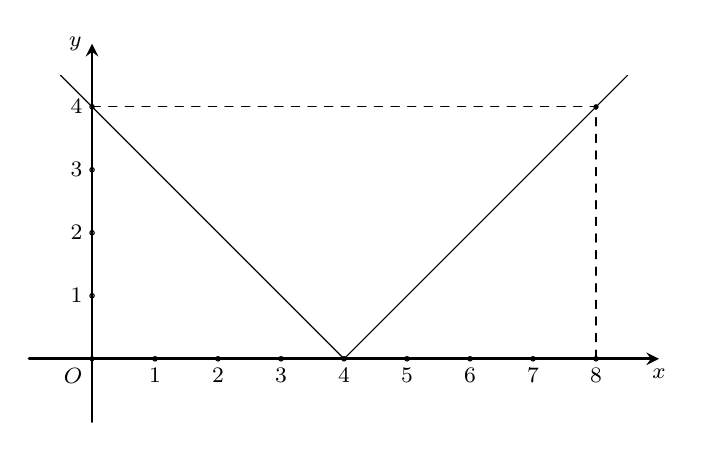
\begin{tikzpicture}[>=stealth,line join=round,line cap=round,font=\footnotesize,scale=0.8]
					\draw[->,line width = 1pt] (-1,0)--(9,0) node[below]{$x$};
					\fill (0,0) node[below left]{$O$} circle (1.2 pt);
					\draw[->,line width = 1pt] (0,-1) --(0,5) node[left]{$y$};
					\foreach \x in {1,2,3,4,5,6,7,8}{
						\draw (\x,0) node[below]{$\x$} circle (1pt);
					}
					\foreach \x in {1,2,3,4}{
						\draw (0,\x) node[left]{$\x$} circle (1pt);
					}
					\draw[dashed] (0,4)--(8,4)--(8,0);
					\draw [domain=-0.5:4, samples=100] %
					plot (\x, {(-1*(\x)+4)});
					\draw [domain=4:8.5, samples=100] %
					plot (\x, {((\x)-4)});
					\fill (8,4) circle(1.2pt);
				\end{tikzpicture}
			\end{center}
		\end{itemchoice}
	}
\end{ex}

\begin{ex}%[0D3V1-7]%[Dự án đề cương 2025]%[Mui Doan]
	Một người lái xe trên đường cao tốc với tốc độ trung bình $v$ (km/h). Quãng đường $S$ (km) mà xe đi được trong $t$ giờ được biểu diễn bởi $S(t) = v \cdot t$. Biết $v$ là một hằng số dương. 
	\choiceTF
	{Hàm số $S(t)$ là hàm số bậc hai theo $t$}
	{\True Hàm số $S(t)$ là hàm số đồng biến}
	{\True Nếu người đó đi với tốc độ $80$ km/h trong $2{,}5$ giờ thì quãng đường đi được là $200$ km}
	{\True Đồ thị hàm số $S(t)$ là một đường thẳng đi qua gốc tọa độ}
	\loigiai{
		\begin{itemchoice}
			\itemch Hàm số $S(t)=v \cdot t$ là hàm số bậc nhất theo $t$ (với $v$ là hằng số, đóng vai trò hệ số góc $a$). 
			\itemch Vì $v > 0$, hàm số $S(t)=vt$ có hệ số góc dương, nên nó là hàm số đồng biến.
			\itemch Ta có $S = 80\cdot 2{,}5 = 200$ km. 
			\itemch Hàm số bậc nhất $S(t)=vt$ (với $t \ge 0$) có dạng $y=ax$, là đường thẳng đi qua gốc tọa độ $(0;0)$.
		\end{itemchoice}
	}
\end{ex}

\Closesolutionfile{ans}

\ind{PHẦN III.} \inden{Câu trả lời ngắn.}\\
\setcounter{ex}{0}
\Opensolutionfile{ans}[ans/0D3-Bai1-TLN]%--Đặt tên 2D1-Bai1-DS
\begin{ex}%[0D3H1-3]%[Dự án đề cương 2025]%[Mui Doan]
	Cho hàm số $f(x)=\heva{&x^2+1& \text{khi } x \le 0\\& 2x-3& \text{khi } x > 0}$. Tính giá trị của $f(-2)+f(5)$.
	\par\shortans{12}
	\loigiai{
		Vì $-2\le 0$, ta dùng công thức $f(x)=x^2+1$.\\
		Ta có$f(-2)=(-2)^2+1=5$.\\
		Vì $5> 0$, ta dùng công thức $f(x)=2x-3$.\\
		Ta có $f(5)=2\cdot 5-3=7$.\\
		Vậy $f(-2)+f(5)=5+7=12$.
	}
\end{ex}
\begin{ex}%[0D3H1-5]%[Dự án đề cương 2025]%[Mui Doan]
	Số các giá trị  nguyên dương của tham số $m$ để hàm số $y = (m-3)x + 2$ là hàm số nghịch biến là bao nhiêu?
	\par\shortans{2}
	\loigiai{
		Hàm số $y = (m-3)x + 2$ là hàm số bậc nhất.\\
		Để hàm số bậc nhất nghịch biến, hệ số góc của nó phải âm.\\
		Tức là $m-3 < 0 \Leftrightarrow m < 3$.\\
		Vì $m$ nguyên dương nên $m\in\{1;2\} $.\\
		Suy ra có $2$ giá trị của $m$.
	}
\end{ex}
\begin{ex}%[0D3H1-2]%[Dự án đề cương 2025]%[Mui Doan]
	Tập xác định của hàm số $y = \sqrt{x+3} + \dfrac{1}{x-1}$ là $[a;+\infty)\setminus\{b\}$ với $a$, $b\in\mathbb{Z}$. Tính $a+b$.
	\par\shortans{-2}
	\loigiai{
		Điều kiện $\heva{&x+3 \ge 0\\&x-1 \ne 0}\Leftrightarrow \heva{&x \ge -3\\&x \ne 1.}$\\
		Suy ra tập xác định là $\mathscr{D}=[-3;+\infty)\setminus\{1\}$.\\
		Do đó $a=-3$, $b=1$.\\
		Vậy $a+b=-2$.
	}
\end{ex}

\begin{ex}%[0D3H1-7]%[Dự án đề cương 2025]%[Mui Doan]
	Một người đi xe máy với vận tốc $50$ km/h trong $t$ giờ. Quãng đường người đó đi được là $S(t)$ km. Hỏi quãng đường đi được sau $3$ giờ là bao nhiêu km?
	\par\shortans{150}
	\loigiai{
		Công thức của hàm số biểu diễn quãng đường $S(t)$ là $S(t) = 50t$.\\
		Sau $3$ giờ, quãng đường đi được là $S(3) = 50\cdot 3 = 150$ km.
	}
\end{ex}

\begin{ex}%[0D3H1-7]%[Dự án đề cương 2025]%[Mui Doan]
	Độ cao $h$ (mét) của một viên đạn bay lên theo phương thẳng đứng tại thời điểm $t$ (giây) được cho bởi công thức $h(t) = -4{,}9t^2 + 20t + 2$. Tính độ cao ban đầu của viên đạn.
	\par\shortans{2}
	\loigiai{
		Độ cao ban đầu là độ cao của viên đạn tại thời điểm $t=0$.\\
		Ta có	$h(0) = -4{,}9\cdot 0^2 + 20\cdot 0 + 2=2$.\\
		Vậy độ cao ban đầu của viên đạn là $2$ mét.
	}
\end{ex}
\begin{ex}%[0D3H1-2]%[Dự án đề cương 2025]%[Mui Doan]
	Cho đồ thị hàm số $y=f(x)$ như hình vẽ. Tập xác định của hàm số là $[a;b]$. Tình $2a-3b$.
	\begin{center}
		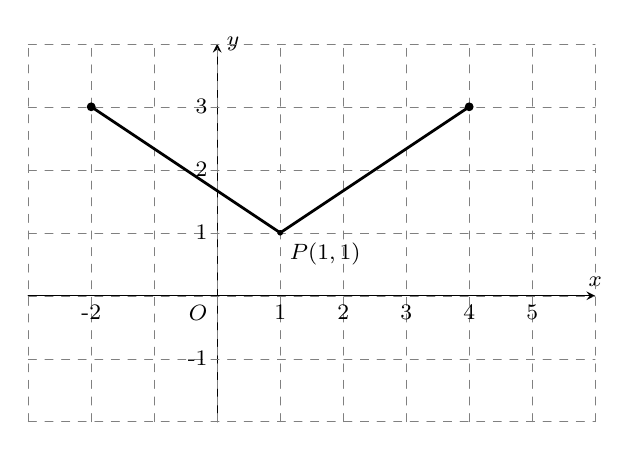
\begin{tikzpicture}[scale=0.8, font=\footnotesize, line join=round, line cap=round, >=stealth]
			\draw[->] (-3,0)--(6,0) node[above]{$x$};
			\draw[->] (0,-2)--(0,4) node[right]{$y$};
			\draw[very thin,step=1cm,color=gray,dashed] (-3,-2)grid(6,4);
			\draw[line width=1pt] (-2,3)--(1,1)--(4,3);
			\fill[black] (-2,3) circle (2pt);
			\fill[black] (4,3) circle (2pt);
			\draw[fill=black] (1,1) circle (1pt) node[below right] {$P(1,1)$};
			\foreach \i in {-2,1,2,3,4,5}
			\draw (\i,0) node[below] {\i};
			\foreach \i in {-1,1,2,3}
			\draw (0,\i) node[left] {\i};
			\node at (0,0) [below left] {$O$};
		\end{tikzpicture}
	\end{center}
	\shortans{8}
	\loigiai{
		Quan sát đồ thị, hàm số được vẽ từ $x=-2$ đến $x=4$.\\
		Tại $x=-2$ và $x=4$, ta thấy hàm số xác định tại các điểm này.\\
		Do đó, tập xác định của hàm số là đoạn $[-2;4]$.\\
		Suy ra $a=-2$, $b=4$.\\
		Vậy $2a-3b=2\cdot (-2)+3\cdot 4=8$.
	}
\end{ex}

\Closesolutionfile{ans}

\ind{PHẦN IV.} \inden{Tự luận.}\\
\setcounter{ex}{0}
\begin{ex}%[0D3N1-2]
	[Trích đề thi giữa học kỳ 2 lớp 10-THPT Lương Ngọc Quyến-Năm học 2023-2024]
	Tập xác định của hàm số $y=\dfrac{3}{3-4x}$ là
	\choice
	{$\mathbb{R}  \setminus \left\{\dfrac{4}{3}\right\}$}
	{$\mathbb{R}  \setminus \left\{-\dfrac{3}{4}\right\}$}
	{\True $\mathbb{R}  \setminus \left\{\dfrac{3}{4}\right\}$}
	{$\left\{\dfrac{3}{4}\right\}$}
	\loigiai{
		Hàm số  xác định khi $3-4x \ne 0 \Leftrightarrow x \ne \dfrac{3}{4}$.\\
		Tập xác định của hàm số $y=\dfrac{3}{3-4x}$ là $\mathscr{D}=\mathbb{R}  \setminus \left\{\dfrac{3}{4}\right\}$.
	}
\end{ex}

\begin{ex}%[0D3N1-2]
	[Trích đề thi học kỳ 1 lớp 10-Sở Nam Định-Năm học 2023-2024]
	Tập xác định của hàm số $y=\dfrac{2023x+2024}{\sqrt{2x^2-5x+2}}$ là
	\choice
	{\True $\left(-\infty;\dfrac{1}{2}\right)\cup(2;+\infty)$}
	{$\left(-\infty;\dfrac{1}{2}\right]\cup[2;+\infty)$}
	{$\left(\dfrac{1}{2};2\right)$}
	{$\left[\dfrac{1}{2};2\right]$}
	\loigiai
	{
		Điều kiện xác định của hàm số đã cho là $2x^2-5x+2>0 \Leftrightarrow \hoac{ & x>2 \\ & x<\dfrac{1}{2}.}$ \\
		Vậy tập xác định của hàm số $y=\dfrac{2023x+2024}{\sqrt{2x^2-5x+2}}$ là $\left(-\infty;\dfrac{1}{2}\right)\cup(2;+\infty)$.
	}
\end{ex}

\begin{ex}%[0D3H1-3]%[Dự án đề cương 2025]%[Mui Doan]
	Cho hàm số $f(x) = 3x^2 - 5x + 2$. Tính giá trị của $f(0)$ và $f(2)$.
	\loigiai{
		Ta có $f(0) = 3\cdot 0^2 - 5\cdot 0 + 2=2$.\\
		$f(2) = 3\cdot 2^2 - 5\cdot 2 + 2=4$.\\
		Vậy $f(0)=2$ và $f(2)=4$.
	}
\end{ex}

\begin{ex}%[0D3H1-5]%[Dự án đề cương 2025]%[Mui Doan]
	Cho hàm số $y = -3x + 7$. Hàm số này đồng biến hay nghịch biến trên $\mathbb{R}$? Giải thích.
	\loigiai{
		Hàm số  bậc nhất có dạng $y=ax+b$ nghịch biến  trên $\mathbb{R}$ khi và chỉ khi $a<0$.\\
		Vì hàm số hàm số $y = -3x + 7$ có  $a=-3 < 0$, nên hàm số $y = -3x + 7$ là hàm số nghịch biến trên $\mathbb{R}$.
	}
\end{ex}
\begin{ex}%[0D3H1-3]%[Dự án đề cương 2025]%[Mui Doan]
	Cho đồ thị hàm số $y=f(x)$ như hình vẽ. Hãy xác định tập giá trị của hàm số.
	\begin{center}
		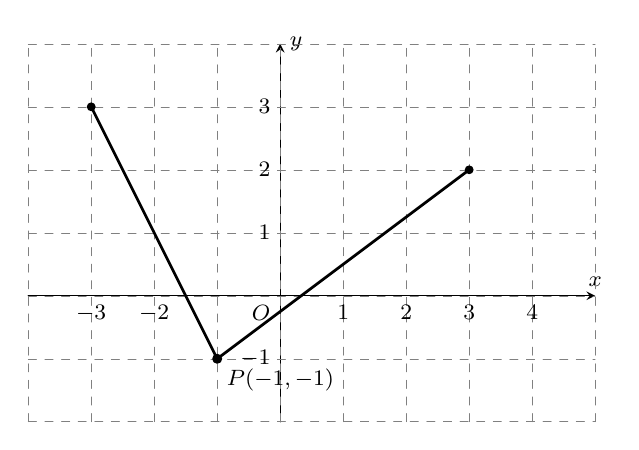
\begin{tikzpicture}[scale=0.8, font=\footnotesize, line join=round, line cap=round, >=stealth]
			\draw[->] (-4,0)--(5,0) node[above]{$x$};
			\draw[->] (0,-2)--(0,4) node[right]{$y$};
			\draw[very thin,step=1cm,color=gray,dashed] (-4,-2)grid(5,4);
			\draw[line width=1pt] (-3,3)--(-1,-1)--(3,2);
			\fill[black] (-3,3) circle (2pt);
			\fill[black] (3,2) circle (2pt);
			\draw[fill=black] (-1,-1) circle (2pt) node[below right] {$P(-1,-1)$};
			\node at (0,0) [below left] {$O$};
			\foreach \i in {-3,-2,1,2,3,4} \draw (\i,0) node[below] {$\i$};
			\foreach \i in {-1,1,2,3} \draw (0,\i) node[left] {$\i$};
		\end{tikzpicture}
	\end{center}
	\loigiai{
		Quan sát đồ thị, giá trị nhỏ nhất của $y$ mà hàm số đạt được là $y=-1$ (tại $x=-1$).\\
		Giá trị lớn nhất của $y$ mà hàm số đạt được là $y=3$ (tại $x=-3$).\\
		Tất cả các giá trị của $y$ mà đồ thị đi qua nằm trong khoảng từ $-1$ đến $3$.\\
		Vậy tập giá trị của hàm số là $[-1;3]$.
	}
\end{ex}
\begin{ex}%[0D3H1-7]%[Dự án đề cương 2025]%[Mui Doan]
	Một công ty điện tử sản xuất một loại linh kiện. Hàm chi phí sản xuất $C(x)$ (triệu đồng) cho $x$ nghìn linh kiện được cho bởi $C(x) = x^2 - 10x + 50$, với $x \in [0, 10]$. Tính chi phí sản xuất $5$ nghìn linh kiện.
	\loigiai{
		 Chi phí sản xuất $5$ nghìn linh kiện (tức $x = 5$):
			$C(5) = 5^2 - 10(5) + 50 = 25 - 50 + 50 = 25$ triệu đồng.
	}
\end{ex}
\begin{ex}%[0D3H1-5]%[Dự án đề cương 2025]%[Mui Doan]
	Tìm tất cả các giá trị của tham số $m$ để hàm số $y = (m-1)x + 2m$ là hàm số đồng biến trên $\mathbb{R}$.
	\loigiai{
		Hàm số $y = (m-1)x + 2m$ là hàm số bậc nhất.\\
		Để hàm số bậc nhất đồng biến trên $\mathbb{R}$,  ta cần 
		$m-1 > 0 \Leftrightarrow m > 1$.\\
		Vậy với $m > 1$, hàm số $y = (m-1)x + 2m$ là hàm số đồng biến trên $\mathbb{R}$.
	}
\end{ex}
\begin{ex}%[0D3H1-7]%[Dự án đề cương 2025]%[Mui Doan]
	Một xe buýt bắt đầu chạy từ một trạm với vận tốc ban đầu là $0$  km/h. Sau khi khởi hành $t$ (phút), vận tốc của xe được cho bởi hàm số $v(t) = 2t + 0{,}1t^2$ (km/h). Tính vận tốc của xe sau $5$ phút khởi hành.
	\loigiai{
		Vận tốc của xe sau $5$ phút khởi hành là $v(5) = 2\cdot 5 + 0{,}1\cdot 5^2=12{,}5$  km/h.
	}
\end{ex}
\begin{ex}%[0D3H1-4]%[Dự án đề cương 2025]%[Mui Doan]
	Vẽ đồ thị hàm số $y = |2x - 4|$. Từ đồ thị, hãy tìm giá trị lớn nhất và nhỏ nhất của hàm số trên đoạn $[0; 3]$.
	\loigiai{
		Ta có thể viết lại hàm số $y = |2x - 4|$ như sau
		$y = |2(x-2)| = 2|x-2|$.
	\[y=\begin{cases} 2(x-2) & \text{khi } x-2\ge 0\\-2(x-2) & \text{khi } x-2< 0\end{cases} \Leftrightarrow y=\begin{cases} 2x-4& \text{khi } x \ge 2\\-2x+4& \text{khi } x < 2.\end{cases}
	\]
	Vẽ đồ thị
	Đồ thị của hàm số là một đường gấp khúc.
	\begin{itemize}
		\item Với $x \ge 2$, đồ thị là đường thẳng $y = 2x - 4$.\\
	Điểm $(2; 0)$ là điểm gãy của đồ thị.
	Chọn thêm điểm: $x=3 \Rightarrow y = 2(3) - 4 = 2$. Điểm $(3; 2)$.
	\item Với $x < 2$, đồ thị là đường thẳng $y = -2x + 4$.
	Chọn thêm điểm: $x=0 \Rightarrow y = -2(0) + 4 = 4$. Điểm $(0; 4)$.
\end{itemize}
	\begin{center}
			\begin{tikzpicture}[line cap=butt,line join=miter,>=stealth]
			\draw[->] (-1.2,0)--(5,0)
			node[shift={(-100:7pt)},font=\normalsize]{$x$};
			\draw[->] (0,-1.2)--(0,5)
			node[shift={(180:7pt)},font=\normalsize]{$y$};
			\draw (5pt,0) |- (0,5pt) (0,0) node[shift={(225:9pt)},font=\normalsize]{$O$};
			\fill (3,2) circle(1pt);
			\draw[dashed] (3,0)--(3,2);
			\foreach \x in {-1,1,2,3,4}{
				\draw (\x,1.5pt)--(\x,-1.5pt) node[font=\scriptsize,shift={(-90:5pt)}]{\x};
			}
			\foreach \y in {-1,1,2,3,4}{
				\draw (1.5pt,\y)--(-1.5pt,\y) node[font=\scriptsize,shift={(180:5pt)}]{\y};
			}
			
			\tikzset{declare function={f(\x)=2*(\x)-4;g(\x)=-2*(\x)+4;}}
			
			\begin{scope}
				\clip (-1.2,-1) rectangle (5,5);
				\draw[samples=100] plot[domain=2:5] (\x, {f(\x)});
				\draw[samples=100] plot[domain=-1.2:2] (\x, {g(\x)});
			\end{scope}
		\end{tikzpicture}
	\end{center}		
		Giá trị lớn nhất và nhỏ nhất trên đoạn $[0; 3]$:
		Theo đồ thị ta có\\
		Giá trị nhỏ nhất của hàm số trên đoạn $[0; 3]$ là $0$, đạt được tại $x=2$.
		Giá trị lớn nhất của hàm số trên đoạn $[0; 3]$ là $4$, đạt được tại $x=0$.
	}
\end{ex}
\begin{ex}%[0D3H1-4]%[Dự án đề cương 2025]%[Mui Doan]
	Cho hàm số $f(x) = |x+3| - |x-1|$.
	\begin{enumerate}
		\item  Viết lại hàm số dưới dạng hàm số xác định theo từng khoảng.
		\item  Vẽ đồ thị hàm số $y = f(x)$.
		\item  Tìm giá trị nhỏ nhất và lớn nhất của hàm số $f(x)$ trên đoạn $[-5; 2]$.
	\end{enumerate}
	\loigiai{
		\begin{enumerate}
			\item Ta xét các khoảng xác định dựa trên các điểm làm cho biểu thức trong dấu giá trị tuyệt đối bằng $0$, đó là $x=-3$ và $x=1$.
		\begin{itemize}
			\item Trường hợp 1: $x < -3$.\\
		$x+3 < 0 \Rightarrow |x+3| = -(x+3)$,\\
		$x-1 < 0 \Rightarrow |x-1| = -(x-1)$.\\
		Suy ra$f(x) = -(x+3) - (-(x-1)) = -x - 3 + x - 1 = -4$.
			\item Trường hợp 2: $-3 \le x < 1$.\\
		$x+3 \ge 0 \Rightarrow |x+3| = x+3$,\\
		$x-1 < 0 \Rightarrow |x-1| = -(x-1)$.\\
		Suy ra $f(x) = (x+3) - (-(x-1)) = x + 3 + x - 1 = 2x + 2$.
			\item Trường hợp 3: $x \ge 1$.\\
		$x+3 > 0 \Rightarrow |x+3| = x+3$,\\
		$x-1 \ge 0 \Rightarrow |x-1| = x-1$.\\
		Suy ra $f(x) = (x+3) - (x-1) = x + 3 - x + 1 = 4$.
	\end{itemize}		
		Vậy hàm số được viết lại là
		\[ f(x) = \begin{cases} -4 & \text{khi } x < -3 \\ 2x + 2 & \text{khi } -3 \le x < 1 \\ 4 & \text{khi } x \ge 1 \end{cases} \]
		\item Vẽ đồ thị hàm số $y = f(x)$
		\begin{center}
				\begin{tikzpicture}[line cap=butt,line join=miter,>=stealth]
				\draw[->] (-5.5,0)--(2.5,0)
				node[shift={(-100:7pt)},font=\normalsize]{$x$};
				\draw[->] (0,-4.2)--(0,5)
				node[shift={(180:7pt)},font=\normalsize]{$y$};
				\draw (5pt,0) |- (0,5pt) (0,0) node[shift={(225:9pt)},font=\normalsize]{$O$};
				\draw[dashed] (1,0)--(1,4) (-3,0)--(-3,-4) (-5,0)--(-5,-4) (2,0)--(2,4);
				\foreach \x in {-4,-2,-1,1,2}{
					\draw (\x,1.5pt)--(\x,-1.5pt) node[font=\scriptsize,shift={(-90:5pt)}]{\x};
				}
				\draw (-3,1.5pt)--(-3,-1.5pt) node[font=\scriptsize,shift={(90:5pt)}]{-3};
				\draw (-5,1.5pt)--(-5,-1.5pt) node[font=\scriptsize,shift={(90:5pt)}]{-5};
				\foreach \y in {-4,-1,1,2,4}{
					\draw (1.5pt,\y)--(-1.5pt,\y) node[font=\scriptsize,shift={(180:5pt)}]{\y};
				}
				
				\tikzset{declare function={f(\x)=-4;g(\x)=2*(\x)+2;h(\x)=4;}}
				
				\begin{scope}
					\clip (-5.5,-4.2) rectangle (5,5);
					\draw[samples=100] plot[domain=-5.5:-3] (\x, {f(\x)});
					\draw[samples=100] plot[domain=-3:1] (\x, {g(\x)});
					\draw[samples=100] plot[domain=1:2.5] (\x, {h(\x)});
				\end{scope}
			\end{tikzpicture}
		\end{center}
		\begin{itemize}
			\item Trên khoảng $(-\infty; -3)$, đồ thị là đường thẳng $y = -4$.
			\item Trên đoạn $[-3; 1)$, đồ thị là đoạn thẳng $y = 2x + 2$.\\
			Tại $x=-3$, $y = 2(-3)+2 = -4$. Điểm $(-3; -4)$.\\
			Tại $x=1$, $y = 2(1)+2 = 4$. Điểm $(1; 4)$.
			\item Trên khoảng $[1; +\infty)$, đồ thị là đường thẳng $y = 4$.
		\end{itemize}		
		Đồ thị là một đường gấp khúc, gồm một tia nằm ngang, một đoạn thẳng dốc lên và một tia nằm ngang khác.		
		\item Theo đồ thị ta có\\
		Giá trị nhỏ nhất của hàm số trên đoạn $[-5; 2]$ là $-4$.\\
		Giá trị lớn nhất của hàm số trên đoạn $[-5; 2]$ là $4$.
	\end{enumerate}
	}
\end{ex}
\begin{ex}%[0D3V1-7]%[Dự án đề cương 2025]%[Mui Doan]
	Một công ty sản xuất đồ chơi ước tính chi phí sản xuất $x$ chiếc xe đồ chơi được cho bởi hàm số $C(x) = 50\,000x + 10\,000\,000$ (đơn vị: đồng). Giá bán mỗi chiếc xe đồ chơi là $150\,000$ đồng.
	\begin{enumerate}
		\item  Viết hàm số $P(x)$ biểu diễn lợi nhuận của công ty khi sản xuất và bán được $x$ chiếc xe đồ chơi.
		\item  Công ty cần sản xuất và bán được bao nhiêu chiếc xe đồ chơi để đạt được lợi nhuận $50\,000\,000$ đồng?
	\end{enumerate}
	\loigiai{
		\begin{enumerate}
			\item 
		Doanh thu khi bán được $x$ chiếc xe đồ chơi là $R(x) = 150\,000x$ (đồng).\\
		Lợi nhuận $P(x) = R(x) - C(x)$.\\
		Ta có $P(x) = 150\,000x - (50\,000x + 10\,000\,000)=100\,000x - 10\,000\,000$ (đơn vị: đồng).
			\item Ta có
			\allowdisplaybreaks
			\begin{align*}
				&P(x) = 50\,000\,000
				\\
				\Leftrightarrow&100\,000x - 10\,000\,000 =50\,000\,000
				\\
				\Leftrightarrow&100\,000x = 60\,000\,000
				\\
				\Leftrightarrow&x = 600.
			\end{align*}
		Vậy công ty cần sản xuất và bán được $600$ chiếc xe đồ chơi để đạt lợi nhuận $50\,000\,000$ đồng.
	\end{enumerate}
	}
\end{ex}
